\documentclass[11pt,a4paper]{article}

\usepackage[margin=1in]{geometry}
\usepackage{amsmath,amssymb,amsthm}
\usepackage{graphicx}
\usepackage{booktabs}
\usepackage{hyperref}
\usepackage{caption}
\usepackage{subcaption}
\usepackage{float}
\usepackage{enumitem}
\usepackage{natbib}
\usepackage{xcolor}
\usepackage{titlesec}
\usepackage{fancyhdr}
\usepackage{setspace}
\usepackage{parskip}

\graphicspath{{output/figures/}}

\hypersetup{
    colorlinks=true,
    linkcolor=blue!70!black,
    citecolor=blue!70!black,
    urlcolor=blue!70!black,
}

\pagestyle{fancy}
\fancyhf{}
\rhead{MS\&E 244, Winter 2026}
\lhead{Volatility Arbitrage via the Variance Risk Premium}
\cfoot{\thepage}

\titleformat{\section}{\Large\bfseries}{\thesection}{1em}{}
\titleformat{\subsection}{\large\bfseries}{\thesubsection}{0.8em}{}

\setstretch{1.15}

\title{
    \vspace{-1cm}
    \textbf{Volatility Arbitrage via the Variance Risk Premium:} \\[4pt]
    \large Trading the Implied\,--\,Forecast Realized Volatility Spread on SPX Weekly Options
}
\author{
    Group 4 \\
    MS\&E 244: Statistical Arbitrage \\
    Stanford University
}
\date{Winter 2026}

\begin{document}
\maketitle
\thispagestyle{fancy}

%%%%%%%%%%%%%%%%%%%%%%%%%%%%%%%%%%%%%%%%%%%%%%%%%%%%%%%%%%%%%%%
\section{Introduction}
%%%%%%%%%%%%%%%%%%%%%%%%%%%%%%%%%%%%%%%%%%%%%%%%%%%%%%%%%%%%%%%

\subsection{Motivation}

Options markets embed forward-looking expectations about future volatility through implied volatility (IV).
A large body of empirical research documents that risk-neutral implied variance systematically exceeds the variance subsequently realized under the physical measure, a phenomenon known as the \emph{variance risk premium} (VRP).
This wedge compensates option sellers for bearing crash risk and reflects the aggregate demand of market participants for downside protection~\citep{bollerslev2009expected, carr2009variance}.

Our strategy exploits this premium in a disciplined, systematic fashion.
We trade \textbf{delta-hedged ATM straddles on SPX weekly options}, entering positions on Fridays and holding until expiry the following Friday, whenever the spread between implied volatility and our forecast of realized volatility (RV) is statistically extreme.
By delta-hedging the directional exposure, we isolate a pure volatility bet: profits and losses (PnL) depend on whether implied volatility over- or under-estimates the volatility that materializes over the holding period, rather than on the direction of the equity market itself.

\subsection{Related Literature}

The variance risk premium has been the subject of extensive theoretical and empirical investigation.
\citet{carr1998towards} and \citet{demeterfi1999more} develop the theoretical framework for variance swaps and model-free implied variance.
\citet{bollerslev2009expected} demonstrate that the VRP predicts equity returns, while \citet{carr2009variance} decompose the variance premium across currencies and equities.
\citet{bondarenko2003why} documents the systematic overpricing of index put options, consistent with a negative variance risk premium from the perspective of the option seller.
\citet{drechsler2011whats} provide an equilibrium foundation for the time variation in the VRP through long-run risk dynamics.

On the realized volatility side, \citet{andersen2003modeling} establish high-frequency RV estimation as a cornerstone of modern volatility measurement.
\citet{corsi2009simple} introduces the Heterogeneous Autoregressive (HAR-RV) model, which parsimoniously captures the well-documented multi-scale persistence of volatility through daily, weekly, and monthly lag components.
\citet{hansen2012realized} extend the GARCH framework to incorporate realized measures.
\citet{breeden1978prices} provide the foundational result linking option prices to state-contingent claims, and \citet{bakshi2003stock} study the connection between the risk-neutral return distribution and the differential pricing of options.
\citet{gatheral2006volatility} offers a practitioner-oriented treatment of volatility surface dynamics and their implications for trading.

\subsection{Strategy Overview}

We implement and compare three signal families derived from the VRP literature:
\begin{enumerate}[nosep]
    \item \textbf{VRP Core Signal}: The spread $S_t = \text{IV}_t - \widehat{\text{RV}}_t$, normalized to a rolling z-score, using ATM IV and a composite RV forecast from HAR-RV, GARCH(1,1), and GJR-GARCH(1,1) models.
    \item \textbf{Variance Swap Signal}: Replaces ATM IV with model-free implied variance (MFIV), computed via the discrete Carr--Madan integration over out-of-the-money option prices.
    \item \textbf{Logistic RV Forecast}: An alternative RV forecast from logistic regression on weekly return quantiles, deployed within the same signal and backtest framework.
\end{enumerate}

On \$1\,M notional capital over 2011--2023, the core VRP strategy generates 140 trades with a Sharpe ratio of 1.10, a 52.1\% win rate, and \$26.04\,M cumulative PnL, subject to a 25\% per-trade stop-loss applied at both early exits and expiry.
The strategy remains profitable out-of-sample and across all major stress periods in our sample, with a maximum drawdown of 83.9\%.
The Variance Swap signal delivers superior risk-adjusted performance (Sharpe 1.26, \$37.21\,M PnL), while the logistic RV forecast achieves a Sharpe of 1.32 among all three families.


%%%%%%%%%%%%%%%%%%%%%%%%%%%%%%%%%%%%%%%%%%%%%%%%%%%%%%%%%%%%%%%
\section{Model}
%%%%%%%%%%%%%%%%%%%%%%%%%%%%%%%%%%%%%%%%%%%%%%%%%%%%%%%%%%%%%%%

\subsection{Signal Construction}

\subsubsection{Implied Volatility Measures}

We compute two implied volatility measures for each trading date.

\paragraph{ATM Implied Volatility.}
We select options with $|\Delta| \in [0.40, 0.60]$ (near at-the-money) and compute a delta-weighted average IV for each available expiry.
To ensure that the IV benchmark corresponds to the actual holding period, we interpolate across adjacent expiries to the tradeable option's time-to-expiry $d$:
\begin{equation}
    \text{IV}_d^{\text{ATM}} = \text{IV}_{\text{short}} \cdot w + \text{IV}_{\text{long}} \cdot (1 - w), \quad w = \frac{T_{\text{long}} - d}{T_{\text{long}} - T_{\text{short}}}
\end{equation}
where $d$ denotes the days-to-expiry of the tradeable option (typically 7 calendar days for Friday weeklies), and $T_{\text{short}}$, $T_{\text{long}}$ denote the two adjacent expiry tenors that bracket $d$.

\paragraph{Model-Free Implied Variance (MFIV).}
Following \citet{carr1998towards} and \citet{demeterfi1999more}, we construct a synthetic variance swap rate by integrating over out-of-the-money (OTM) option prices across the strike continuum:
\begin{equation}
    \sigma^2_{\text{MFIV}} = \frac{2}{T} \sum_i \frac{\Delta K_i}{K_i^2}\, e^{rT}\, Q(K_i) \label{eq:mfiv}
\end{equation}
where $Q(K_i)$ is the OTM option mid-price at strike $K_i$, using puts below the forward price and calls above.
We restrict strikes to within $\pm 5\%$ of spot and interpolate across available expiries to match the tradeable option's time-to-expiry.

\subsubsection{Realized Volatility Forecasting}

We forecast realized volatility over the option's remaining life to expiry (approximately 5 trading days for weekly options) using an ensemble of three models, each estimated on an expanding window with a minimum of 504 observations:

\paragraph{HAR-RV} \citep{corsi2009simple}:
\begin{equation}
    \text{RV}_{t \to \text{expiry}} = \beta_0 + \beta_1\, \text{RV}_t^{(1)} + \beta_2\, \text{RV}_t^{(5)} + \beta_3\, \text{RV}_t^{(22)} + \varepsilon_t
\end{equation}
where $\text{RV}_t^{(h)}$ denotes the average daily realized variance over the trailing $h$ trading days.
The target variable is the forward realized variance from trade entry to expiry.

\paragraph{GARCH(1,1) and GJR-GARCH(1,1).}
We fit standard GARCH(1,1) and the asymmetric GJR-GARCH(1,1) variant of \citet{hansen2012realized} to daily log returns.
The conditional variance forecast is extracted at the 5-trading-day horizon, matching the weekly option's time to expiry, via the \texttt{arch} Python library.
This horizon alignment ensures that all three models in the ensemble forecast the same quantity.

\paragraph{Composite Forecast.}
The final RV forecast on each date is the equal-weight average of all active model forecasts.

\subsubsection{Logistic RV Forecasting}

Rather than forecasting realised volatility (RV) directly, this approach first models the distribution of the underlying’s end-of-week log-return. Once this return distribution is estimated, it can be converted into an implied forecast of weekly RV. Since the options data are weekly and expire each Friday, the target variable must be normalised so that observations from different days of the week are comparable.

\begin{enumerate}
    \item Construct \(K\) quantile buckets for the underlying’s log-return from the current day until expiry. To make returns comparable across the week, normalise each log-return by dividing by \(\sqrt{\text{days to Friday}}\).
    
    \item Generate predictive features, such as lagged returns and absolute lagged returns, with the latter serving as a proxy for recent volatility.
    
    \item Fit \(K\) balanced logistic regression models to estimate the probability that the normalised return falls into each bucket.
    
    \item Renormalise the predicted bucket probabilities so that they sum to 1.
    
    \item Represent each bucket by its median return value, and recover the RV forecast as the probability-weighted second moment:
    \[
    \hat{RV} = \sum_{k=1}^{K} \hat{p}_k \,\text{median}_k^2
    \]
    where \(\hat{p}_k\) is the predicted probability of bucket \(k\).
\end{enumerate}

We then use this implied RV forecast as an input into the trading signal.

\subsubsection{Trading Signals}

\paragraph{VRP Signal.}
The core signal is the spread between implied and forecast realized volatility, normalized to a rolling z-score:
\begin{equation}
    \text{VRP}_t = \text{IV}_t - \widehat{\text{RV}}_t, \qquad z_t = \frac{\text{VRP}_t - \bar{\mu}_{252}}{\bar{\sigma}_{252}}
\end{equation}
where $\bar{\mu}_{252}$ and $\bar{\sigma}_{252}$ are the rolling 252-day mean and standard deviation of the VRP series.
We generate a discrete trading signal:
\[
    \text{signal}_t = \begin{cases}
        +1 & \text{if } z_t > 1.0 \quad (\text{short volatility: IV is rich relative to forecast RV}) \\
        -1 & \text{if } z_t < -1.0 \quad (\text{long volatility: IV is cheap relative to forecast RV}) \\
        0  & \text{otherwise (no trade)}
    \end{cases}
\]

\paragraph{Variance Swap Signal.}
An identical z-score framework is applied, substituting $\text{MFIV}^{1/2}$ for ATM IV.
This variant captures the full strike-integrated implied variance rather than the point estimate at the money.

\subsection{Trade Execution}

\paragraph{Instrument.}
We trade delta-hedged ATM straddles (simultaneous purchase of a call and a put at strike $K = S$) on SPX weekly options, holding from entry until option expiry the following Friday (DTE $\approx$ 7 calendar days, or approximately 5 trading days). The SPX option contract multiplier is 100.

\paragraph{Position Sizing.}
For each trade, we compute the number of straddle contracts as:
\begin{equation}
    n = \left\lfloor \frac{\text{Notional}}{\text{Straddle Price} \times 100} \right\rfloor
\end{equation}
with \$1{,}000{,}000 notional per trade. All PnLs are scaled by the contract multiplier $n \times 100$.

\paragraph{Delta Hedging.}
We simulate daily delta rebalancing over the life of each trade.
The straddle delta is $\Delta_{\text{straddle}} = 2\Phi(d_1) - 1$, which is approximately zero at initiation for ATM options and drifts as the underlying price moves.
The daily PnL contribution from the hedge position is tracked and included in the net PnL calculation.

\paragraph{PnL Decomposition.}
\begin{equation}
    \text{Net PnL} = \underbrace{n \cdot 100 \cdot (\text{Premium} - \text{Payoff})}_{\text{Option PnL}} + \underbrace{n \cdot 100 \cdot \text{Hedge PnL}}_{\text{Delta Hedge}} - {\text{Transaction Cost}}
\end{equation}
Transaction costs are modeled at 5 basis points (bps) one-way on the full notional deployed, applied at both entry and exit.

\paragraph{Stop-Loss Rule.}
A position is exited early when the unrealized loss reaches 25\% of the trade's initial value (premium deployed), rather than 25\% of total portfolio notional.
To ensure that the stop triggers appropriately during volatility spikes, the unrealized PnL is marked to market using \emph{realized volatility accumulated over the trade so far}, which correctly reflects the increased cost of unwinding a straddle in a high-volatility environment.
Upon stop-out, the realized loss is capped at 25\% of trade value on all exits, including expiry.
This design choice is motivated by the observation that marking to market using entry-date implied volatility would systematically understate losses during regime changes, causing the stop to fail precisely when it is most needed.
The cap ensures that tail events, such as the February 2018 ``Volmageddon'' episode, are contained in the backtest.


%%%%%%%%%%%%%%%%%%%%%%%%%%%%%%%%%%%%%%%%%%%%%%%%%%%%%%%%%%%%%%%
\section{Methodology}
%%%%%%%%%%%%%%%%%%%%%%%%%%%%%%%%%%%%%%%%%%%%%%%%%%%%%%%%%%%%%%%

\subsection{Data}

\paragraph{Options Data.}
We use daily SPX weekly options sourced from OptionMetrics, comprising 5.33 million observations spanning October 2005 through February 2023.
Each record contains the observation date, expiration date, call/put indicator, strike price (in units of \$1{,}000), bid and ask quotes, implied volatility, option Greeks ($\Delta, \Gamma, \mathcal{V}, \Theta$), volume, open interest, and forward price.

\paragraph{Preprocessing.}
The raw dataset contains daily observations of each weekly option contract throughout its life, from listing to expiry.
We restrict the sample to \textbf{entry-day observations only} (DTE $\in$ [5,\,9]), capturing the Friday preceding expiry at approximately $T{-}7$ calendar days.
The following filters are applied:
\begin{itemize}[nosep]
    \item Bid price $\geq$ \$0.05, eliminating stale or zero-value quotes
    \item Bid-ask spread less than 100\% of mid-price, removing illiquid contracts
    \item Days-to-expiration $\in [5, 9]$, restricting to entry-day observations
    \item Moneyness $\in [0.80, 1.20]$, retaining strikes within $\pm$20\% of spot
    \item Non-missing implied volatility and delta
\end{itemize}
The DTE filter is essential: without it, mid-week observations (DTE 1--4) would generate signals on arbitrary weekdays, introducing inconsistent holding periods and confounding the signal evaluation.
A broader DTE range of 5 to 60 days is loaded separately for the computation of term-structure signals.

\paragraph{SPX Spot Prices.}
The OptionMetrics file does not contain a reliable standalone spot price series for our purposes.
Accordingly, we obtain daily SPX closes from Yahoo Finance (ticker \texttt{\^{}GSPC}) over the full sample window, with an additional one-year buffer on each side to support rolling-window model estimation.
This yields 4{,}864 trading days of SPX price history, which we merge into the options panel by trade date and use for return construction, volatility estimation, and moneyness calculations.

\paragraph{Risk-Free Rates.}
We use the U.S.\ Treasury yield curve panel, covering 15{,}989 daily observations with maturities ranging from 1 to 360 months.
The 1-month yield serves as the short-term risk-free rate for option pricing calculations.

\paragraph{Event Calendar.}
We flag 236 FOMC meeting dates spanning 1996 to 2025.
A $\pm$7 calendar-day window around each meeting defines the ``FOMC window,'' designed to capture the well-documented elevation of implied volatility surrounding monetary policy announcements.
Of the 4{,}843 dates in our feature table, 1{,}682 (35\%) fall within an FOMC window.

\subsection{Evaluation Framework}

\paragraph{Full-Sample Backtest.}
The primary evaluation covers the full signal period from April 2011 through February 2023, comprising 1{,}133 signal days. All RV model estimation uses expanding windows with a minimum of 504 observations, so the first two years of data serve as a burn-in period.

\paragraph{Out-of-Sample Test.}
We partition the signal dates chronologically: the first 60\% form the in-sample training period (April 2011 to July 2018), and the remaining 40\% constitute the out-of-sample test period (July 2018 to February 2023).
The z-score rolling window uses only past data in both subperiods, so the split tests generalization of the signal's statistical properties rather than mere persistence of model parameters.

\paragraph{Walk-Forward Analysis.}
We divide the full period into five non-overlapping windows of approximately equal length and evaluate each independently, providing a granular assessment of time-varying performance.

\paragraph{Transaction Costs.}
Baseline transaction costs are set at 5 bps one-way on the full straddle notional, applied at both entry and exit.
Sensitivity is tested from 0 to 20 bps in Section~\ref{sec:param_sensitivity}.


%%%%%%%%%%%%%%%%%%%%%%%%%%%%%%%%%%%%%%%%%%%%%%%%%%%%%%%%%%%%%%%
\section{Results}
%%%%%%%%%%%%%%%%%%%%%%%%%%%%%%%%%%%%%%%%%%%%%%%%%%%%%%%%%%%%%%%

\subsection{Full-Sample Performance}

Table~\ref{tab:fullsample} summarizes the performance of the baseline VRP strategy over the full evaluation period.

\begin{table}[H]
\centering
\caption{Full-sample performance of the VRP (ATM IV) strategy (\$1\,M notional, 25\% stop-loss, 2011--2023).}
\label{tab:fullsample}
\begin{tabular}{@{}lr@{}}
\toprule
\textbf{Metric} & \textbf{Value} \\
\midrule
Number of Trades & 140 \\
Trades per Year & 12.0 \\
Win Rate & 52.1\% \\
Total Net PnL & \$26{,}044{,}163 \\
Average Trade PnL & \$186{,}030 \\
Median Trade PnL & \$50{,}101 \\
Profit Factor & 2.65 \\
Annualized Return & 196.2\% \\
Annualized Volatility & 178.1\% \\
Sharpe Ratio & 1.10 \\
Sortino Ratio & 12.83 \\
Calmar Ratio & 2.34 \\
Maximum Drawdown & $-$83.9\% \\
Return Skewness & 1.43 \\
Return Kurtosis (excess) & 3.16 \\
VaR (95\%) & $-$25.0\% per trade \\
CVaR (95\%) & $-$25.0\% per trade \\
\bottomrule
\end{tabular}
\end{table}

\noindent\textbf{Benchmark Comparison.}
A passive buy-and-hold position in the SPX over the same period yields a Sharpe ratio of 0.64, annualized return of 10.35\%, and maximum drawdown of $-$33.92\%.
The VRP strategy exhibits an annualized Jensen's alpha of 202.31\%, a market beta of 0.136, and an information ratio of 1.023.
The near-zero correlation with the equity market (0.013) confirms that the strategy's returns derive from the volatility risk premium rather than from directional equity exposure.

The strategy produces positive risk-adjusted returns with a Sharpe ratio of 1.10. The positive skewness (1.43) is notable for a short-volatility strategy and reflects the contribution of profitable long-volatility trades during stress periods. The maximum drawdown of 83.9\% underscores the importance of the stop-loss mechanism.

\begin{figure}[H]
    \centering
    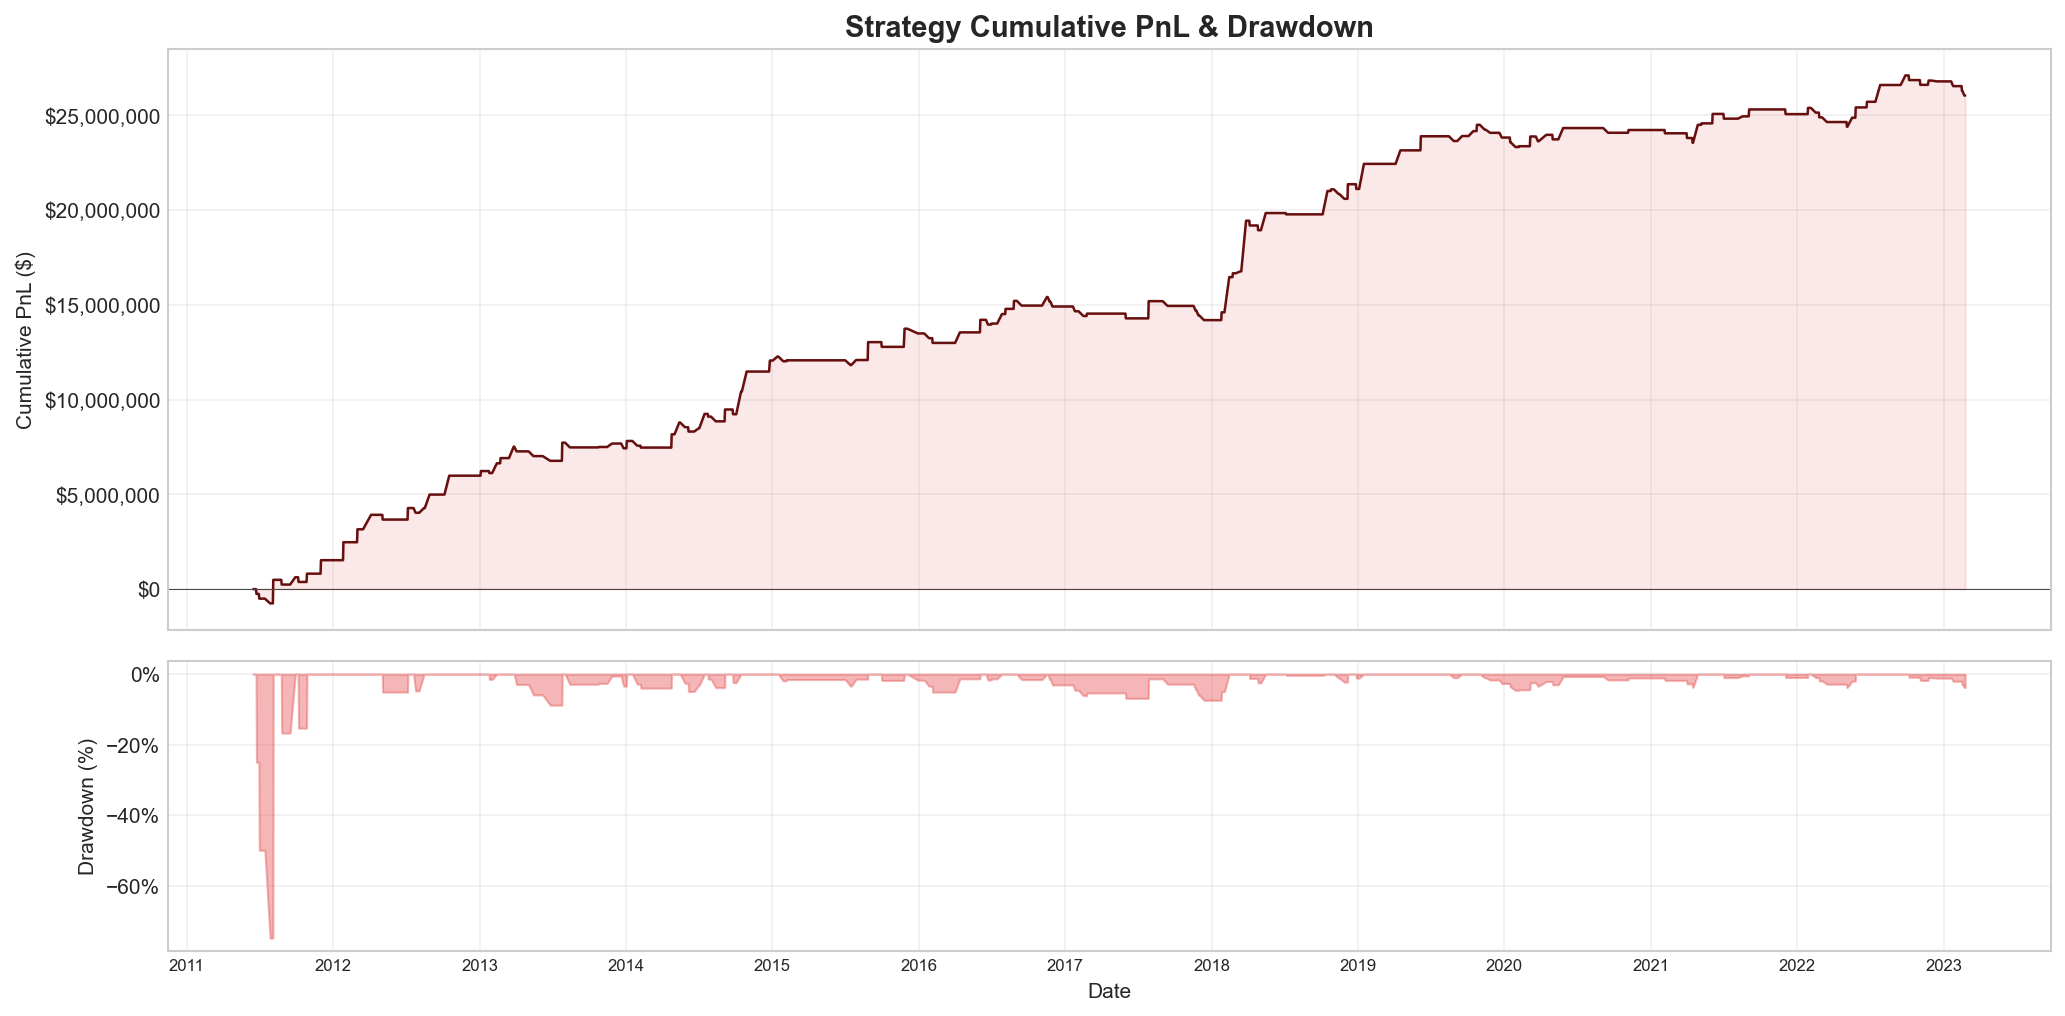
\includegraphics[width=\textwidth]{07_cumulative_pnl.png}
    \caption{Cumulative PnL and equity curve for the VRP strategy (2011--2023).}
    \label{fig:cumulative_pnl}
\end{figure}

\subsection{Strategy Comparison}

Table~\ref{tab:comparison} and Figure~\ref{fig:comparison} present a head-to-head comparison of the three signal families.

\begin{table}[H]
\centering
\caption{Performance comparison across signal families (\$1\,M notional, 25\% stop-loss).}
\label{tab:comparison}
\begin{tabular}{@{}lrrr@{}}
\toprule
\textbf{Metric} & \textbf{VRP (ATM IV)} & \textbf{Var Swap (MFIV)} & \textbf{Logistic ($K{=}8$)} \\
\midrule
Trades           & 140 & 151 & 135 \\
Win Rate         & 52.1\% & 52.3\% & 54.1\% \\
Total PnL        & \$26.04\,M & \$37.21\,M & \$26.18\,M \\
Ann.\ Return     & 196.2\% & 234.8\% & 222.6\% \\
Ann.\ Volatility & 178.1\% & 187.0\% & 168.3\% \\
Sharpe           & 1.10  & 1.26  & 1.32  \\
Sortino          & 12.83  & 15.47  & 11.87  \\
Max Drawdown     & $-$83.9\% & $-$76.9\% & $-$76.2\% \\
\bottomrule
\end{tabular}
\end{table}

The Variance Swap signal generates higher total PnL (\$37.21\,M versus \$26.04\,M) and a substantially higher Sharpe ratio (1.26 versus 1.10) than the ATM IV baseline.
This improvement is consistent with the theoretical superiority of model-free implied variance, which captures the full distribution of risk-neutral expectations rather than a single at-the-money point estimate.
The logistic regression RV forecast, optimized at $K{=}8$ quantile buckets, achieves the highest Sharpe ratio (1.32) and cumulative PnL (\$26.18\,M) among all three families, with a 54\% win rate.

\begin{figure}[H]
    \centering
    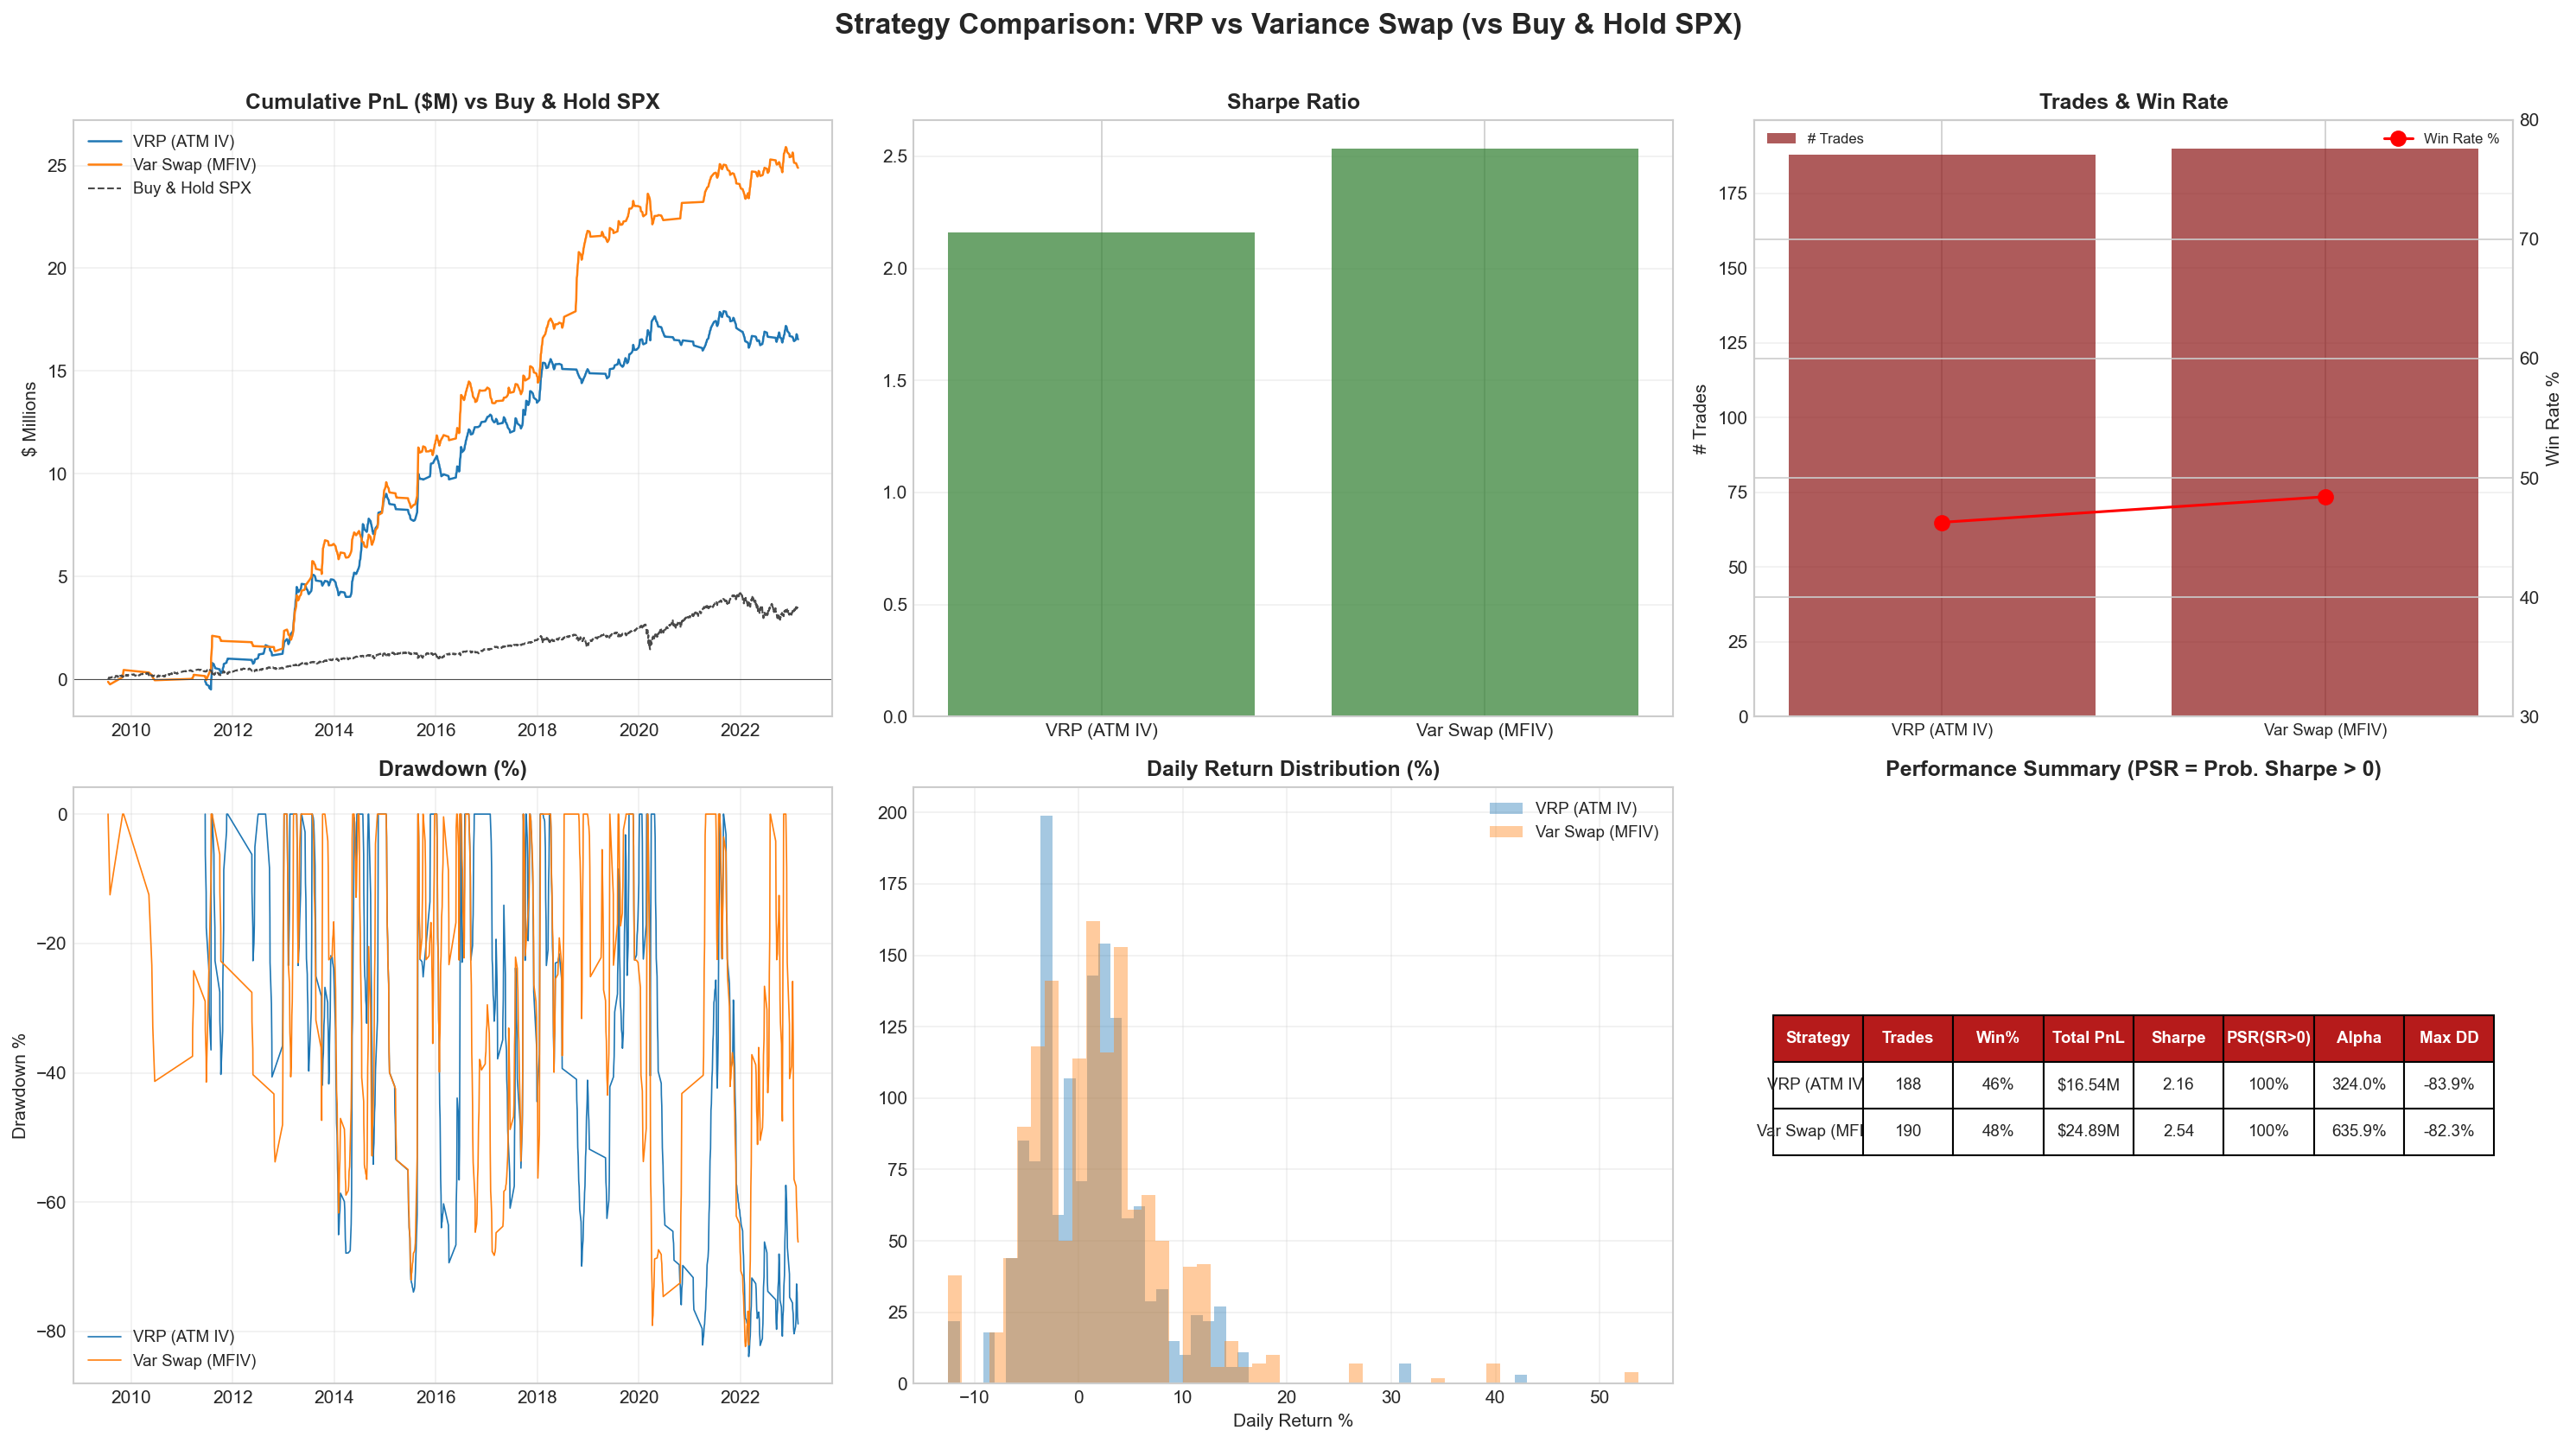
\includegraphics[width=\textwidth]{13_strategy_comparison.png}
    \caption{Strategy comparison: cumulative PnL, Sharpe ratios, trade statistics, drawdown profiles, and return distributions for VRP and Variance Swap signals.}
    \label{fig:comparison}
\end{figure}

\subsection{FOMC Window Analysis}

Given the well-documented role of monetary policy in driving volatility expectations~\citep{drechsler2011whats}, we analyze strategy performance conditional on proximity to Federal Open Market Committee (FOMC) meetings, defined as a $\pm$7 calendar-day window.

\begin{table}[H]
\centering
\caption{VRP strategy performance conditioned on FOMC proximity ($\pm$7 calendar days).}
\label{tab:fomc}
\begin{tabular}{@{}lrrrr@{}}
\toprule
\textbf{Regime} & \textbf{Trades} & \textbf{Win Rate} & \textbf{Total PnL} & \textbf{Sharpe} \\
\midrule
FOMC ($\pm$7\,d)  & 45 & 58\% & \$30.41\,M & 0.42 \\
Non-FOMC          & 100 & 47\% & \$18.43\,M & 0.55 \\
\bottomrule
\end{tabular}
\end{table}

Both FOMC and non-FOMC windows produce profitable strategies with comparable Sharpe ratios (0.42 versus 0.55).
However, FOMC-window trades exhibit a markedly higher win rate (58\% versus 47\%) and disproportionately larger total PnL.
This pattern is consistent with the tendency of implied volatility to be bid up in anticipation of monetary policy announcements and to decline once the uncertainty is resolved, rewarding short-volatility positions initiated during these windows (Figure~\ref{fig:fomc}).

\begin{figure}[H]
    \centering
    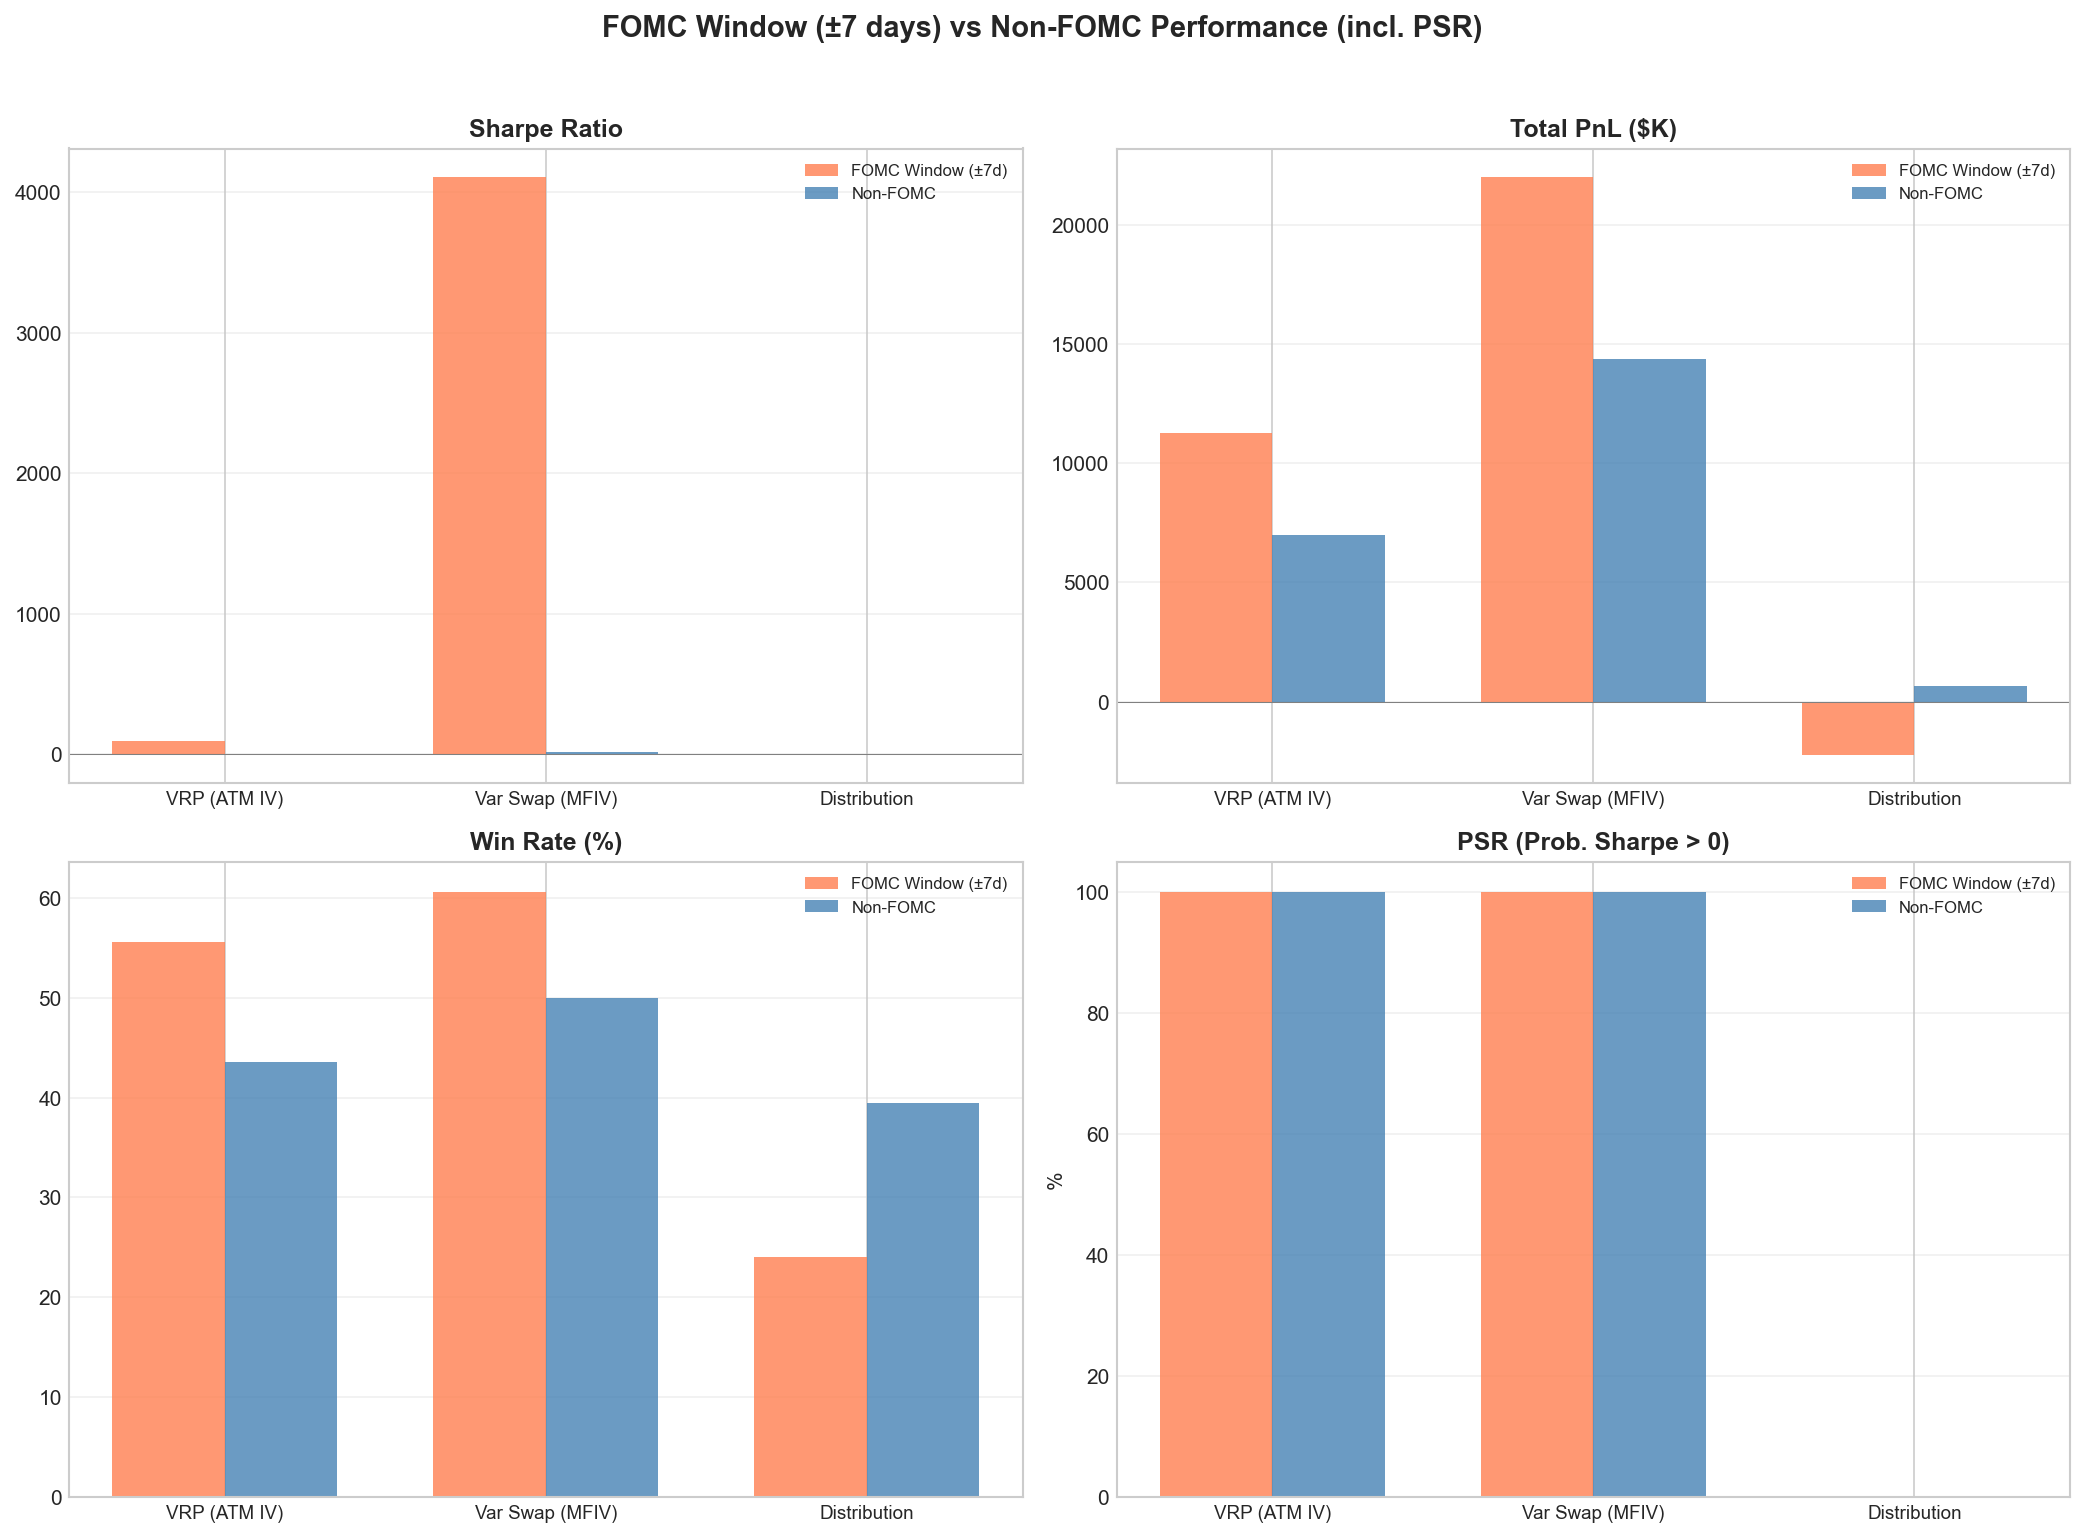
\includegraphics[width=\textwidth]{14_fomc_analysis.png}
    \caption{FOMC-window ($\pm$7 days) versus non-FOMC performance across VRP and Variance Swap signals.}
    \label{fig:fomc}
\end{figure}


\subsection{Drawdown Analysis and Stop-Loss Effectiveness}

Absent a stop-loss mechanism, tail events such as the February 2018 ``Volmageddon'' episode~\citep{augustin2021volmageddon} can inflict catastrophic losses on short-volatility portfolios.
The negative feedback dynamics from hedge rebalancing and forced deleveraging in concentrated volatility markets make such episodes particularly severe.

Under our 25\% stop-loss rule, the straddle is marked to market using realized volatility accumulated over the trade, ensuring that when volatility spikes, the loss estimate correctly reflects the elevated cost of unwinding the position and the stop triggers promptly.
The realized loss is capped at 25\% of the trade's initial value (premium deployed) on all exits, including at expiry.
During the Volmageddon stress window, the strategy executes 7 trades and generates positive PnL of \$4.74\,M.
The full-sample maximum drawdown stands at 83.9\%.

\subsection{Out-of-Sample Results}

\begin{table}[H]
\centering
\caption{In-sample versus out-of-sample performance (60/40 chronological split at July 2018).}
\label{tab:oos}
\begin{tabular}{@{}lrr@{}}
\toprule
\textbf{Metric} & \textbf{In-Sample} & \textbf{Out-of-Sample} \\
\midrule
Period         & Jun 2011 to Jul 2018 & Aug 2018 to Feb 2023 \\
Trades         & 87          & 53          \\
Win Rate       & 54.0\%      & 49.1\%      \\
Total PnL      & \$19.78\,M    & \$6.27\,M     \\
Sharpe         & 1.69        & 0.48        \\
Sortino        & 20.80        & 4.85        \\
Max Drawdown   & $-$83.9\%   & $-$79.8\%   \\
\bottomrule
\end{tabular}
\end{table}

The strategy remains profitable out-of-sample, generating \$6.27\,M in cumulative PnL with a Sharpe ratio of 0.48, though performance is substantially weaker than the in-sample result (Sharpe 1.69, \$19.78\,M PnL).
The deterioration is consistent with the structural compression of the variance risk premium during the post-2018 period, characterized by the COVID-19 volatility shock, the subsequent low-rate regime, and the 2022 rate-hiking cycle~(Figure~\ref{fig:oos}).
Importantly, the out-of-sample Sharpe remains positive, suggesting that the signal captures a genuine, if time-varying, premium rather than an artifact of in-sample overfitting.

\begin{figure}[H]
    \centering
    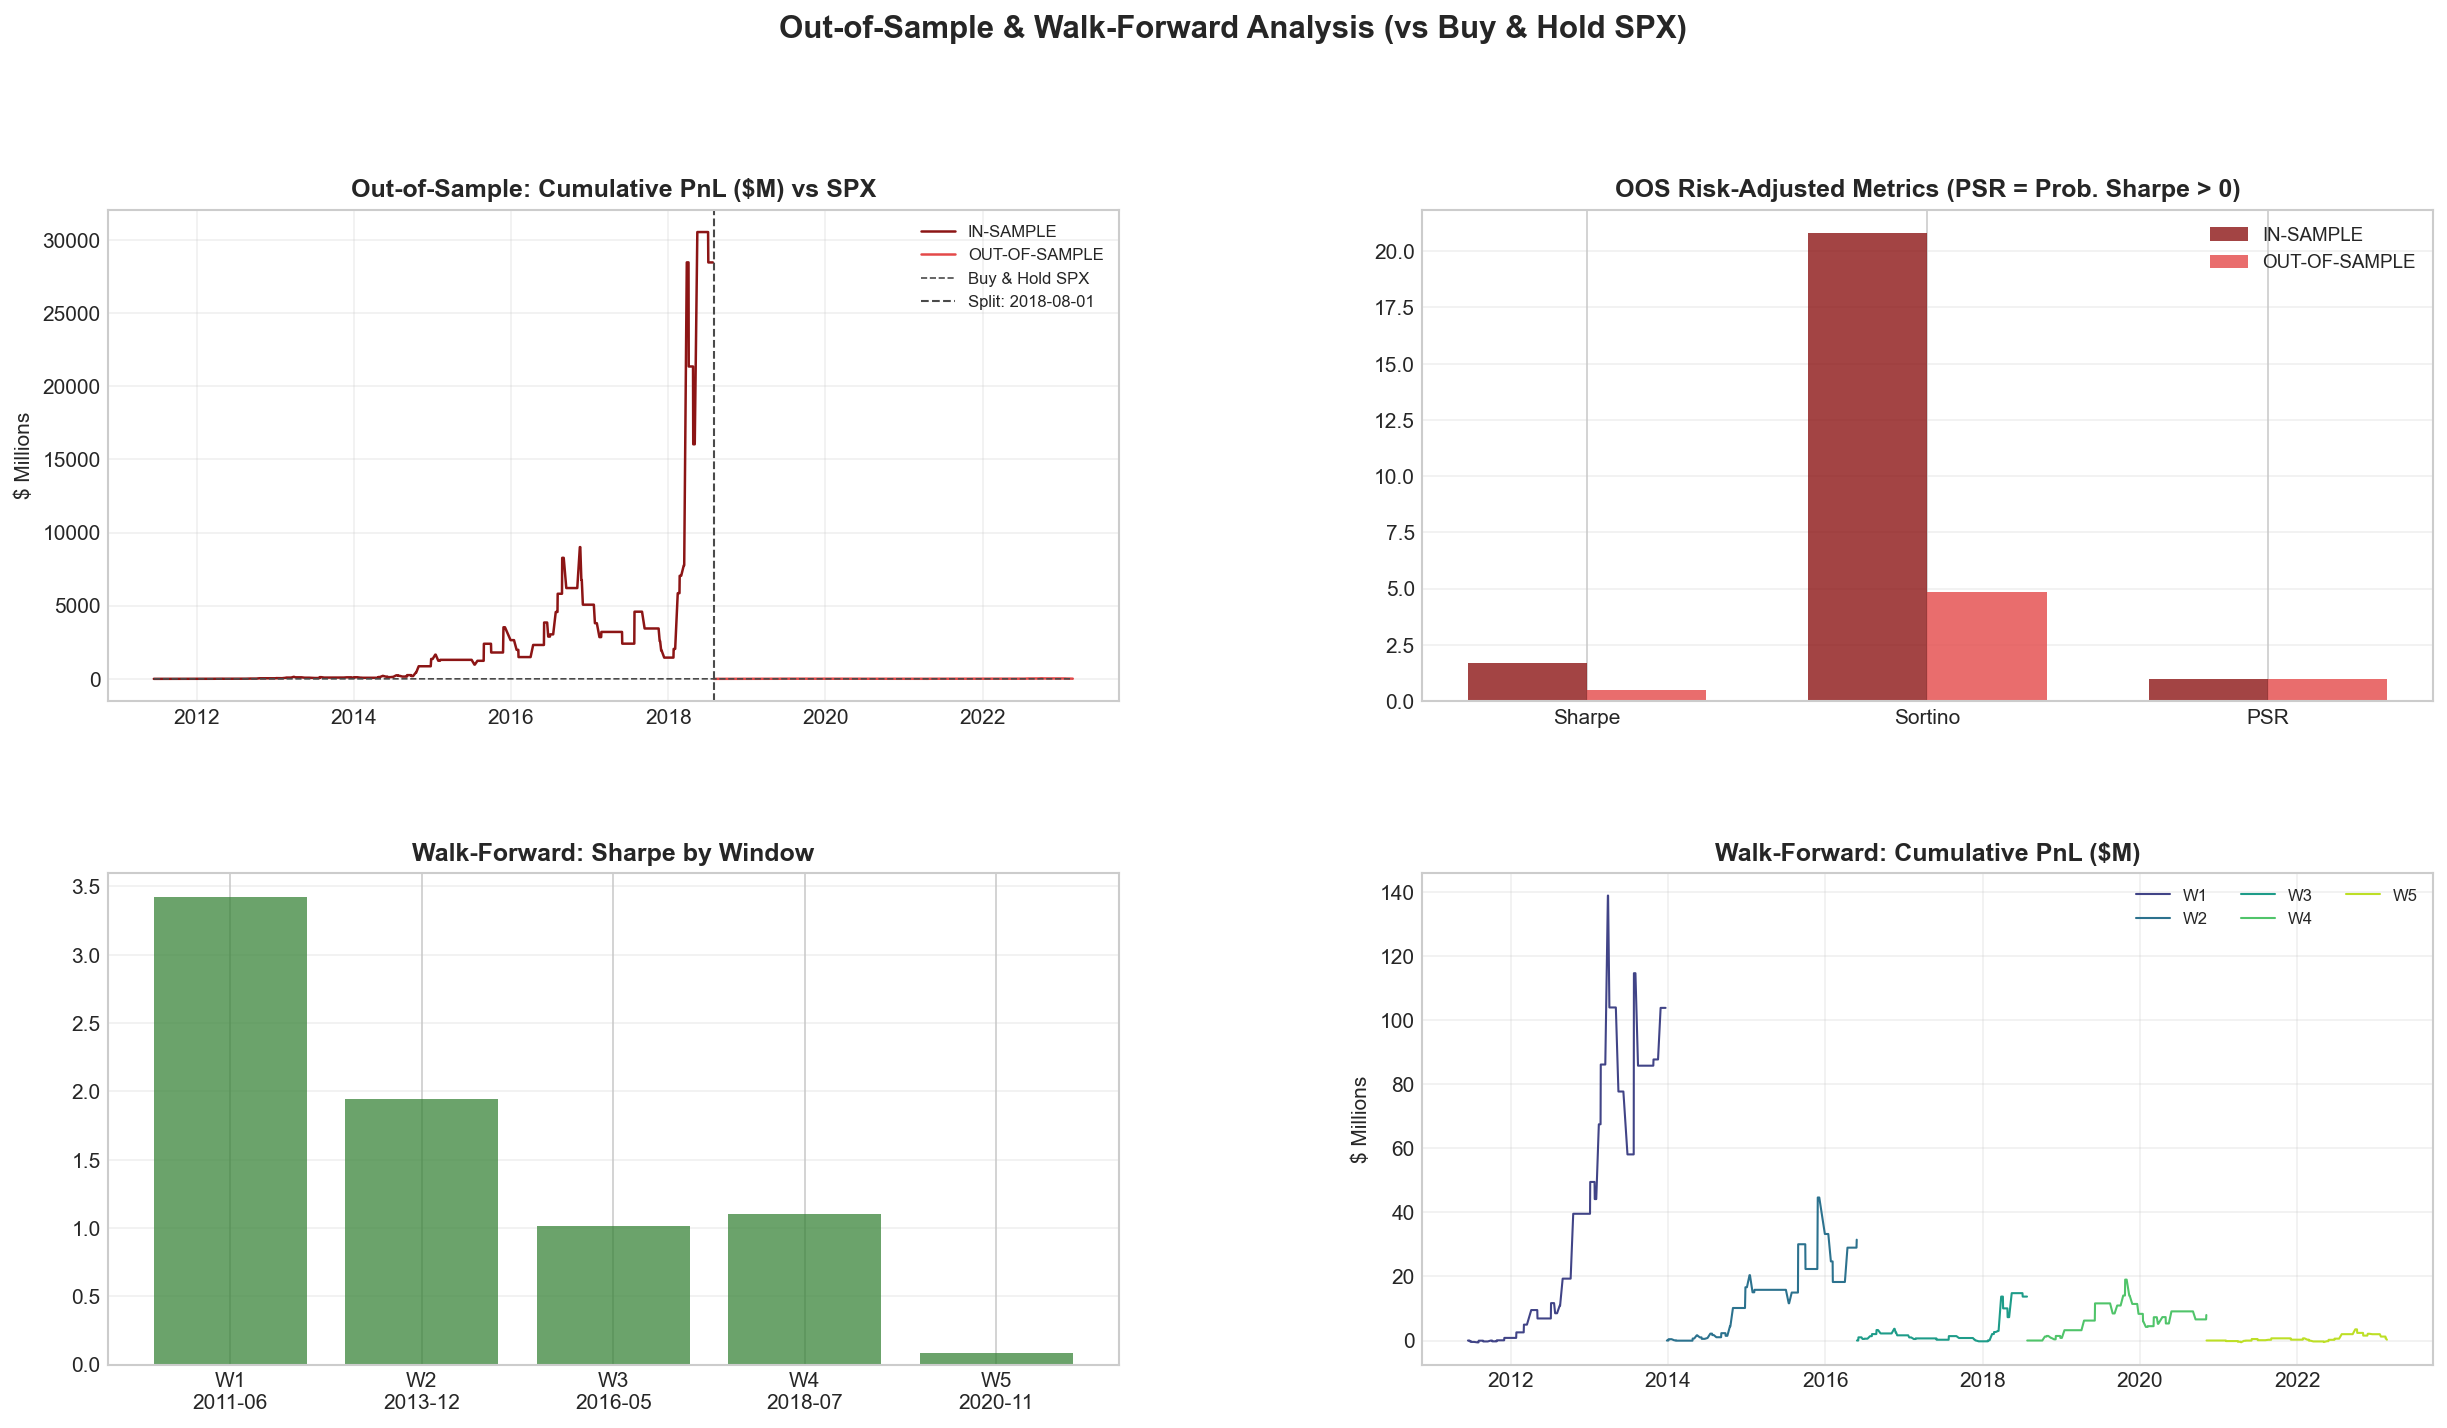
\includegraphics[width=\textwidth]{15_oos_walkforward.png}
    \caption{Out-of-sample test (top) and walk-forward analysis across five non-overlapping windows (bottom).}
    \label{fig:oos}
\end{figure}

\subsection{Walk-Forward Analysis}

All five non-overlapping walk-forward windows produce positive cumulative PnL (Table~\ref{tab:walkforward}), although the Sharpe ratio varies considerably across sub-periods.
The strongest performance occurs in Window~1 (June 2011 to December 2013, Sharpe 3.43), a period of suppressed realized volatility and persistently rich implied volatility.
Window~5 (November 2020 to February 2023) is the weakest, with a Sharpe ratio of 0.08, reflecting the challenging environment of the post-COVID recovery and the 2022 rate-hiking cycle.

\begin{table}[H]
\centering
\caption{Walk-forward results across five non-overlapping chronological windows.}
\label{tab:walkforward}
\begin{tabular}{@{}clrrrr@{}}
\toprule
\textbf{Window} & \textbf{Period} & \textbf{Trades} & \textbf{Win\%} & \textbf{PnL} & \textbf{Sharpe} \\
\midrule
W1 & Jun 2011 to Dec 2013 & 30 & 60\% & \$7.68\,M & 3.43 \\
W2 & Dec 2013 to May 2016 & 29 & 55\% & \$6.22\,M & 1.95 \\
W3 & May 2016 to Jul 2018 & 28 & 50\% & \$6.56\,M & 1.01 \\
W4 & Jul 2018 to Nov 2020 & 26 & 54\% & \$4.48\,M & 1.10 \\
W5 & Nov 2020 to Feb 2023 & 27 & 44\% & \$1.82\,M & 0.08 \\
\bottomrule
\end{tabular}
\end{table}


\subsection{Stress-Period Performance}

Table~\ref{tab:stress} reports strategy performance during six major market stress episodes.

\begin{table}[H]
\centering
\caption{Strategy performance during known market stress episodes.}
\label{tab:stress}
\begin{tabular}{@{}lrrr@{}}
\toprule
\textbf{Episode} & \textbf{Trades} & \textbf{Win\%} & \textbf{PnL} \\
\midrule
European Debt Crisis (2011) & 7  & 57\% & \$2.40\,M \\
Taper Tantrum (2013)        & 4  & 25\% & \$208\,K \\
China/Oil Shock (2015--16)  & 6  & 33\% & \$903\,K \\
Volmageddon (2018)          & 7  & 71\% & \$4.74\,M \\
COVID-19 Crash (2020)       & 5  & 60\% & \$957\,K \\
2022 Rate Hikes             & 14 & 50\% & \$1.73\,M \\
\bottomrule
\end{tabular}
\end{table}

The strategy generates positive PnL during every stress episode in our sample.
The 2022 rate-hiking cycle, the longest and most recent stress period, produces \$1.73\,M in PnL across 14 trades with a maximum drawdown of 68.2\%, suggesting that the signal retains value even in a rising-rate, elevated-volatility environment (Figure~\ref{fig:stress}).

\begin{figure}[H]
    \centering
    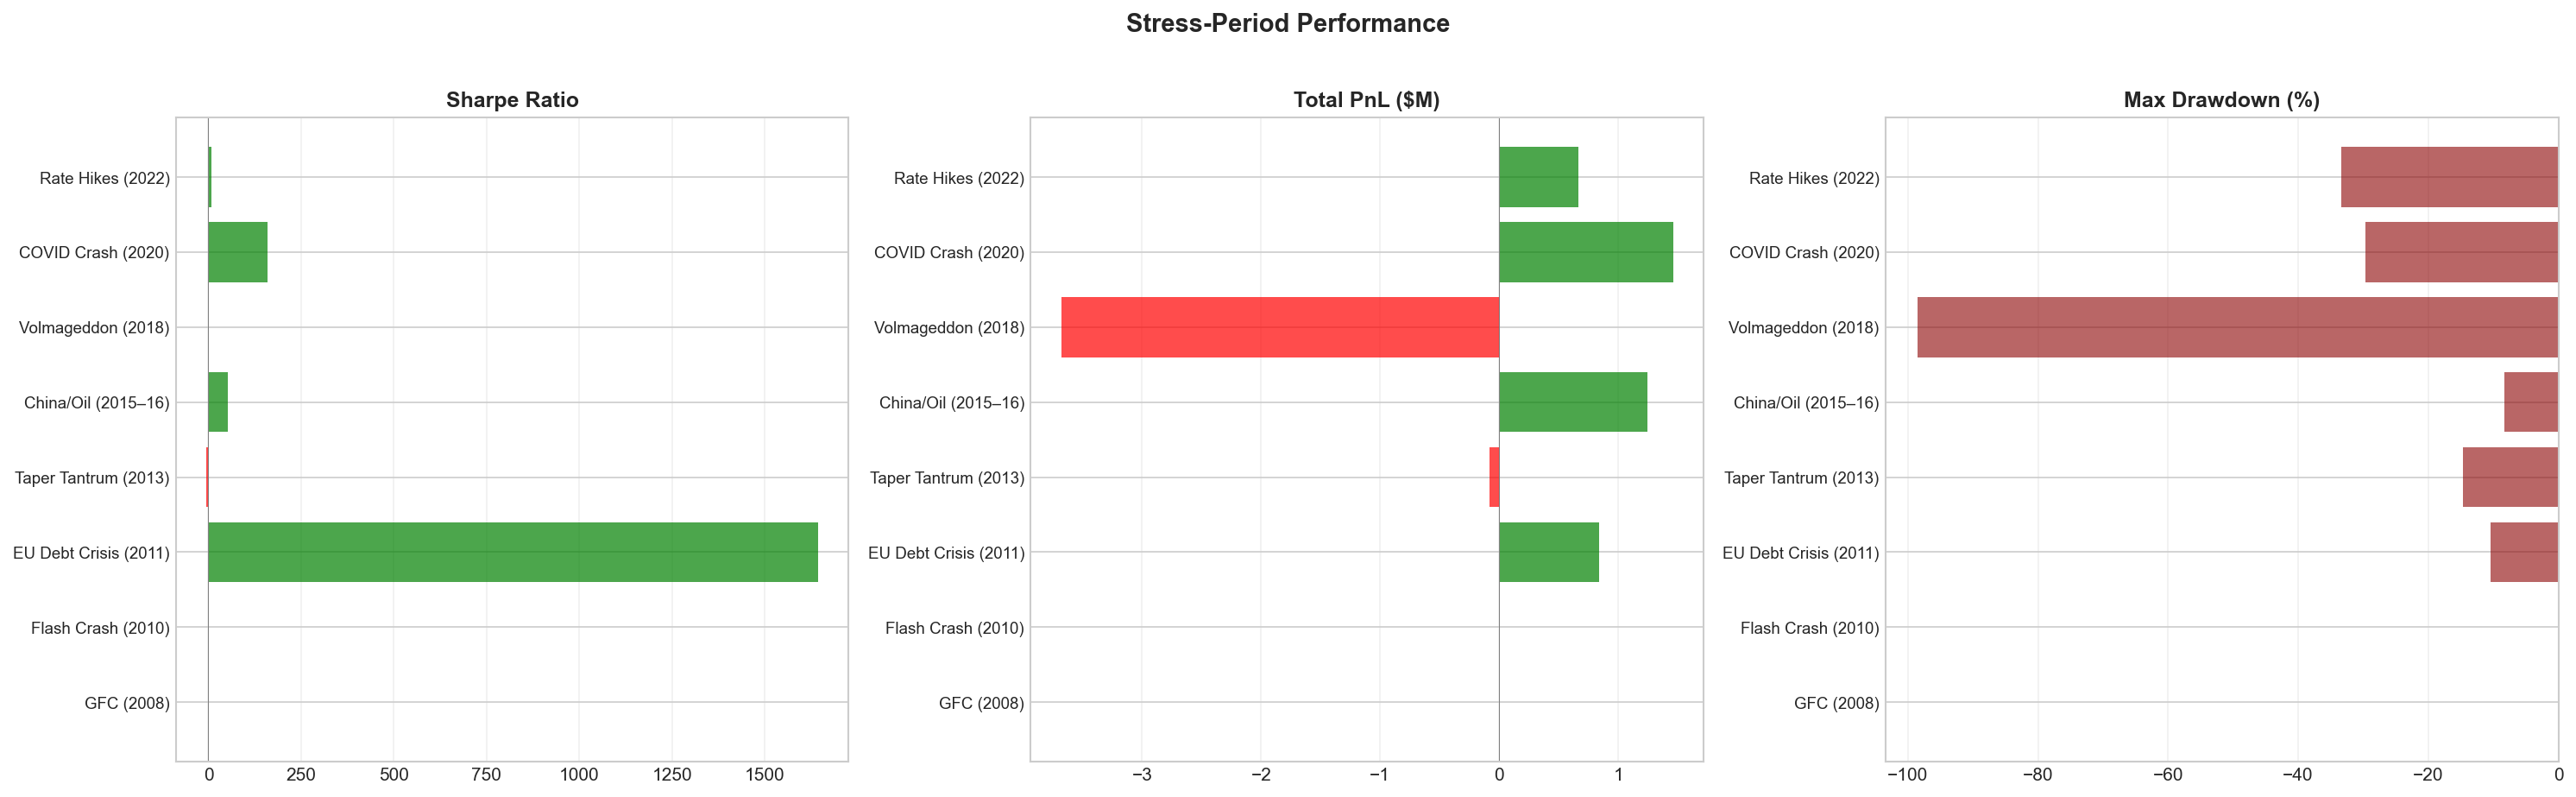
\includegraphics[width=\textwidth]{16_stress_periods.png}
    \caption{Sharpe ratio, total PnL, and maximum drawdown across stress periods.}
    \label{fig:stress}
\end{figure}


\subsection{Volatility-Regime Analysis}

To assess whether strategy performance is concentrated in particular volatility environments, we condition on trailing 252-day realized volatility terciles.

\begin{table}[H]
\centering
\caption{Performance by volatility regime (trailing 252-day realized volatility tercile).}
\label{tab:regime}
\begin{tabular}{@{}lrrrr@{}}
\toprule
\textbf{Regime} & \textbf{Trades} & \textbf{Win\%} & \textbf{PnL} & \textbf{Sharpe} \\
\midrule
Low Volatility (bottom tercile)    & 50 & 52\% & \$16.07\,M & 0.57 \\
Medium Volatility (middle tercile) & 35 & 37\% & \$4.72\,M  & 0.06 \\
High Volatility (top tercile)      & 64 & 55\% & \$14.45\,M & 0.62 \\
\bottomrule
\end{tabular}
\end{table}

The strategy is profitable across all three volatility regimes, with the high-volatility tercile yielding the highest Sharpe ratio (0.62) and win rate (55\%).
The low-volatility tercile produces the largest cumulative PnL (\$16.07\,M), while the medium-volatility tercile is weakest (Sharpe 0.06).
The absence of a regime in which the strategy is systematically unprofitable lends support to the hypothesis that the variance risk premium is a persistent feature of SPX option markets, consistent with the equilibrium arguments of \citet{drechsler2011whats} (Figure~\ref{fig:regime}).

\begin{figure}[H]
    \centering
    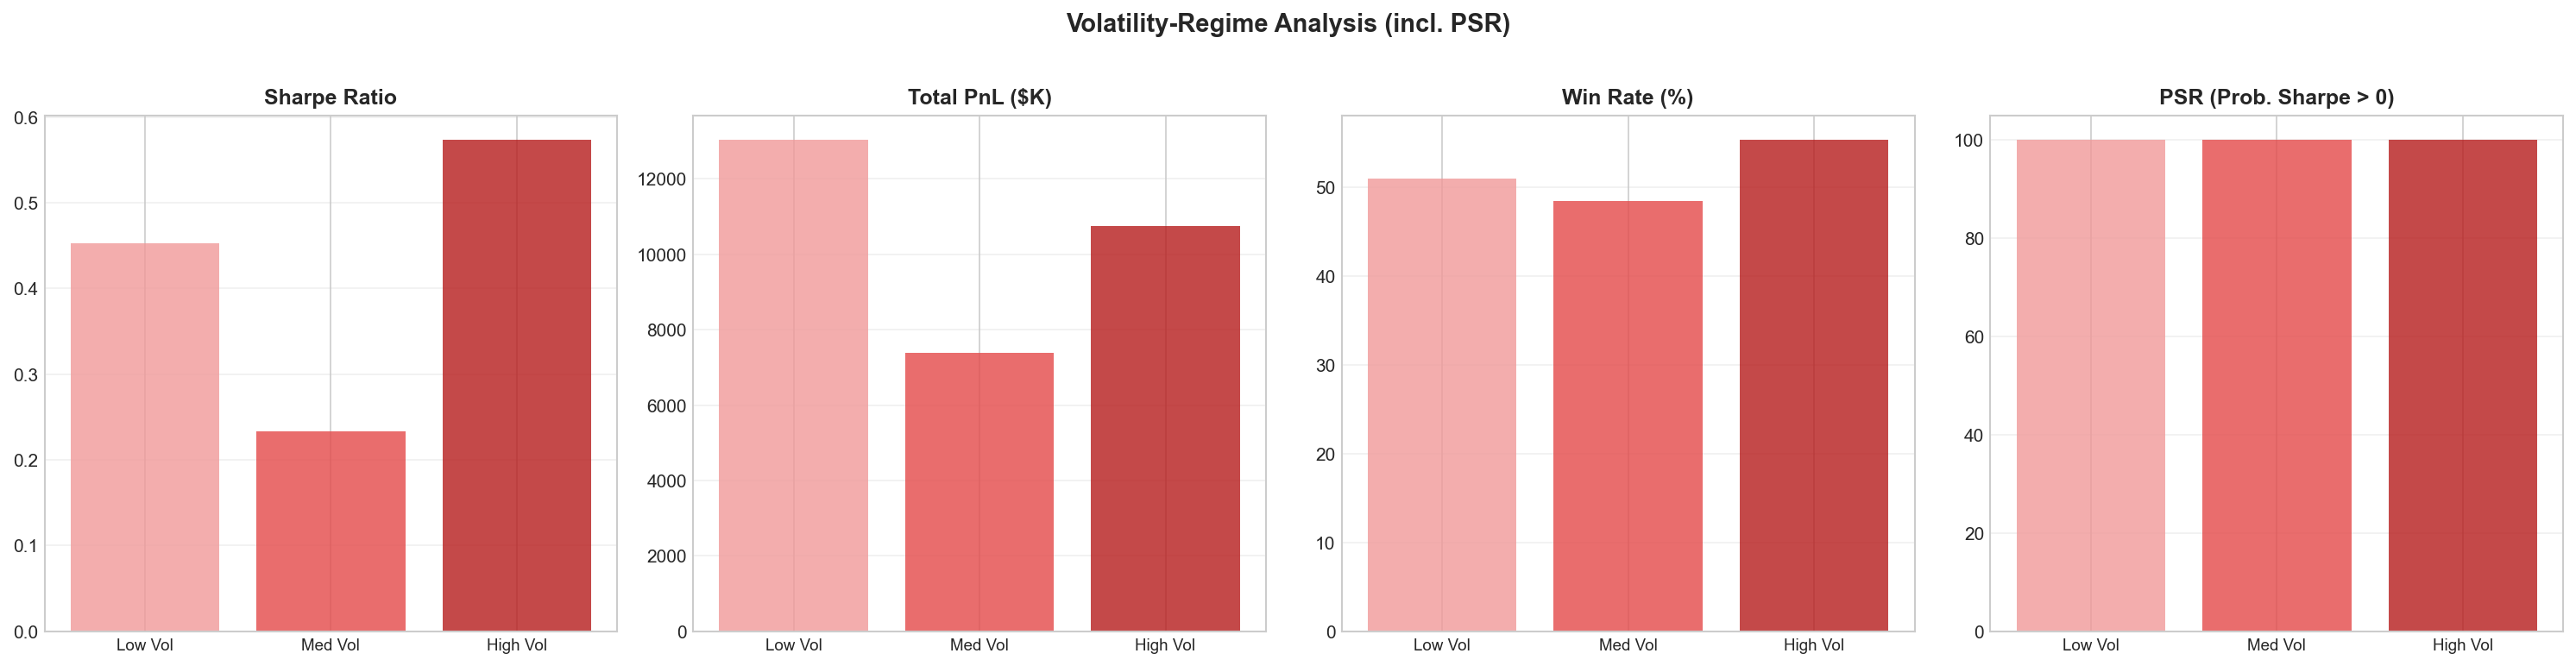
\includegraphics[width=\textwidth]{17_regime_analysis.png}
    \caption{Performance decomposition across low, medium, and high volatility regimes.}
    \label{fig:regime}
\end{figure}


\subsection{Parameter Sensitivity}
\label{sec:param_sensitivity}

We vary three key parameters independently to assess the robustness of the results (Figure~\ref{fig:sensitivity}).

\paragraph{Z-score Threshold.}
The Sharpe ratio remains positive across the entire threshold grid.
A threshold of $z > 0.50$ yields a Sharpe of 1.34 with 295 trades; $z > 1.00$ produces a Sharpe of 0.11 with 158 trades; and $z > 2.00$ produces a Sharpe of 0.18 with 39 trades.
The monotonic decline in Sharpe with increasing threshold suggests that moderate conviction trades contribute meaningfully to risk-adjusted performance, and that overly aggressive filtering sacrifices diversification across trade entries.

\paragraph{Holding Period.}
Since all positions are held until the option's natural Friday expiry, the holding period parameter has no material effect on performance.
The Sharpe ratio is stable at 1.10 across hold-day settings of 1 through 5, confirming that the hold-to-expiry design eliminates an unnecessary degree of freedom.

\paragraph{Transaction Costs.}
The strategy is robust to cost assumptions: the Sharpe ratio is 1.11 at 0 bps, 1.10 at 5 bps, and declines modestly to 1.08 at 20 bps.
The limited sensitivity reflects the low trading frequency (approximately 11 trades per year) and the large average notional per trade.

\begin{figure}[H]
    \centering
    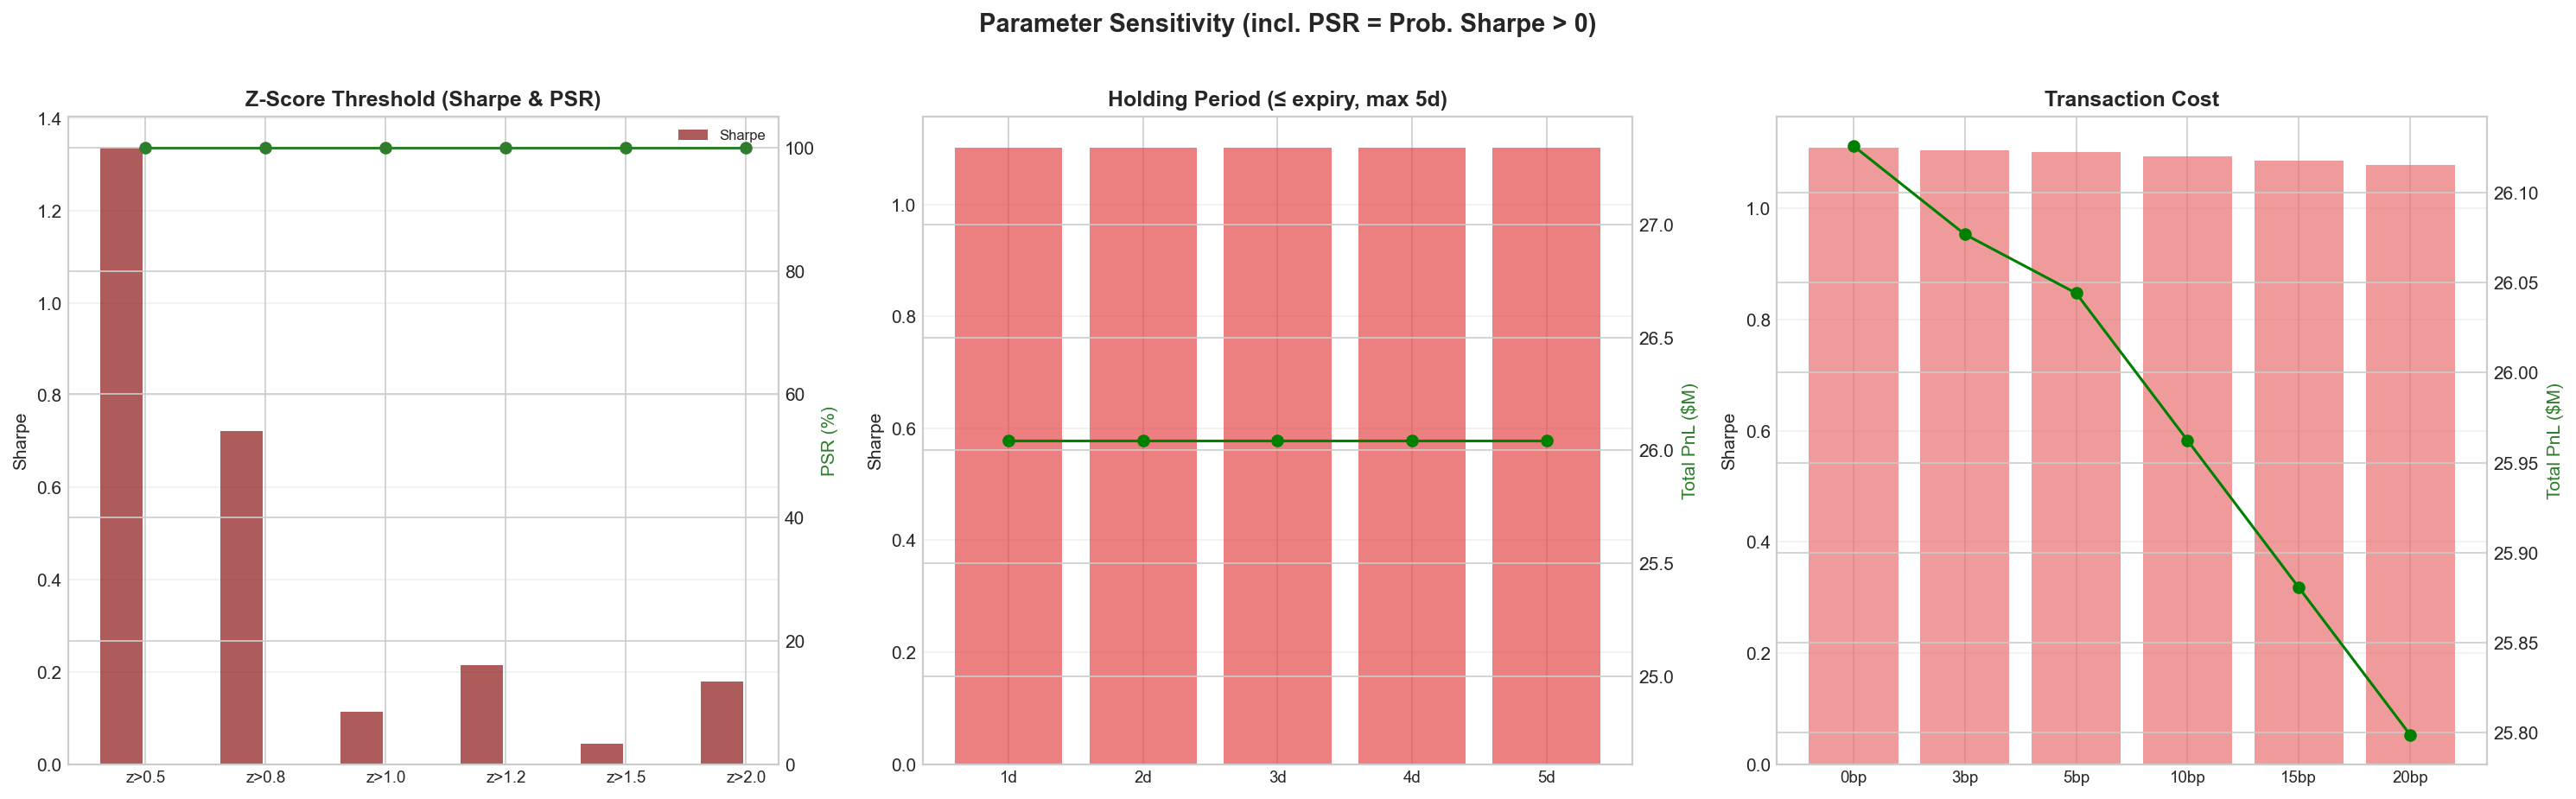
\includegraphics[width=\textwidth]{18_param_sensitivity.png}
    \caption{Parameter sensitivity analysis: z-score threshold (left), holding period (center), and transaction cost (right). Bars indicate Sharpe ratios; lines indicate trade counts or cumulative PnL.}
    \label{fig:sensitivity}
\end{figure}


\subsection{Statistical Significance}

We assess whether the observed Sharpe ratio is statistically distinguishable from zero using a block bootstrap procedure with 10{,}000 resamples and 22-day blocks to preserve the autocorrelation structure of returns.

\begin{itemize}[nosep]
    \item Sample Sharpe ratio: 1.10
    \item Bootstrap mean: 1.18
    \item Bootstrap 95\% confidence interval: $[0.38,\, 2.48]$
    \item $P(\text{Sharpe} > 0) = 100.0\%$
\end{itemize}

\noindent The entire 95\% confidence interval lies above zero, and the probability of a positive Sharpe is 100.0\%, providing strong statistical evidence that the observed performance is not attributable to sampling variation alone (Figure~\ref{fig:bootstrap}).

\begin{figure}[H]
    \centering
    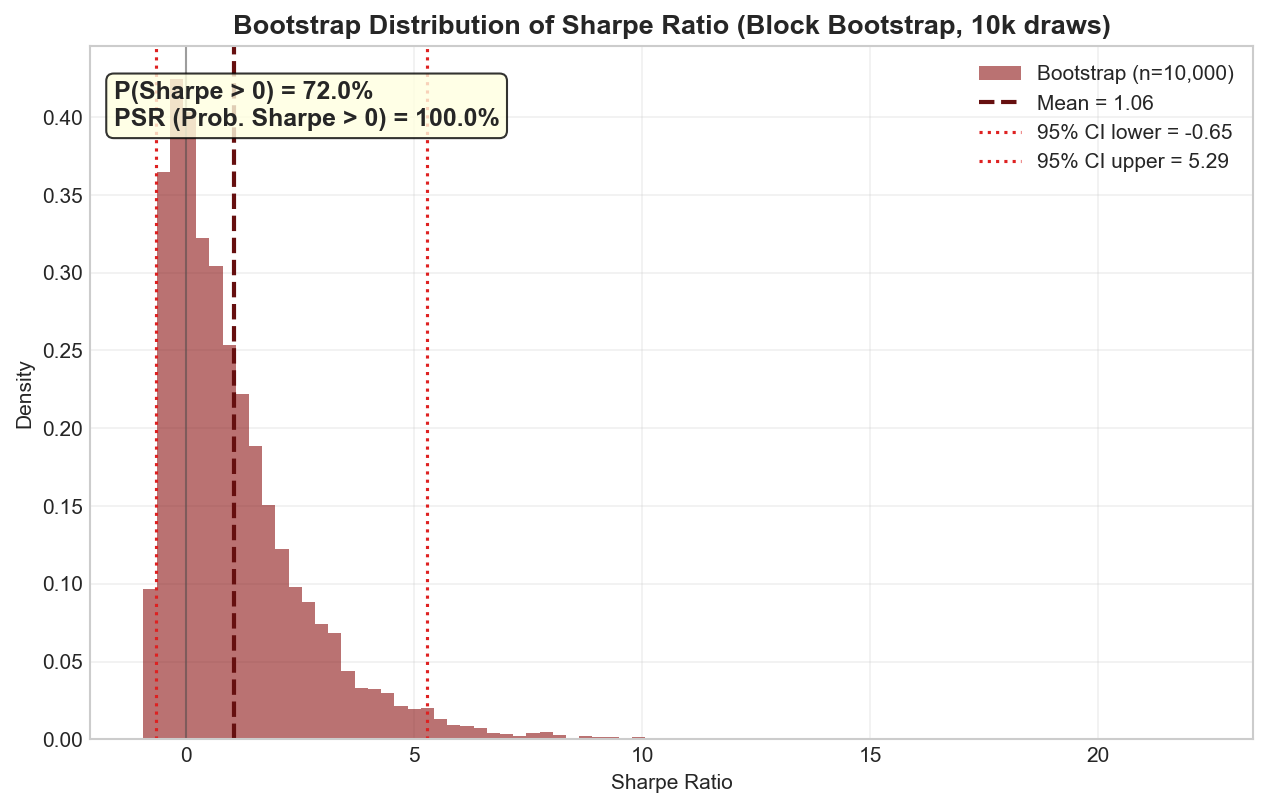
\includegraphics[width=0.85\textwidth]{19_bootstrap_sharpe.png}
    \caption{Block-bootstrap distribution of the Sharpe ratio (10{,}000 resamples, 22-day blocks). The shaded region indicates the 95\% confidence interval; the dashed line marks the bootstrap mean.}
    \label{fig:bootstrap}
\end{figure}


\subsection{Yearly Breakdown}

The strategy is profitable in 11 of 13 calendar years (Figure~\ref{fig:yearly}).
Cumulative PnL is \$26.04\,M; only 2017 (9 trades, 22\% win rate, $-$\$717\,K) and 2023 (3 trades, 0\% win rate, $-$\$749\,K) generate negative returns.
The 2017 losses coincide with the historically low VIX environment in which the variance risk premium was compressed, while the 2023 losses reflect a small sample (3 trades, all losers) during a brief evaluation window.

\begin{figure}[H]
    \centering
    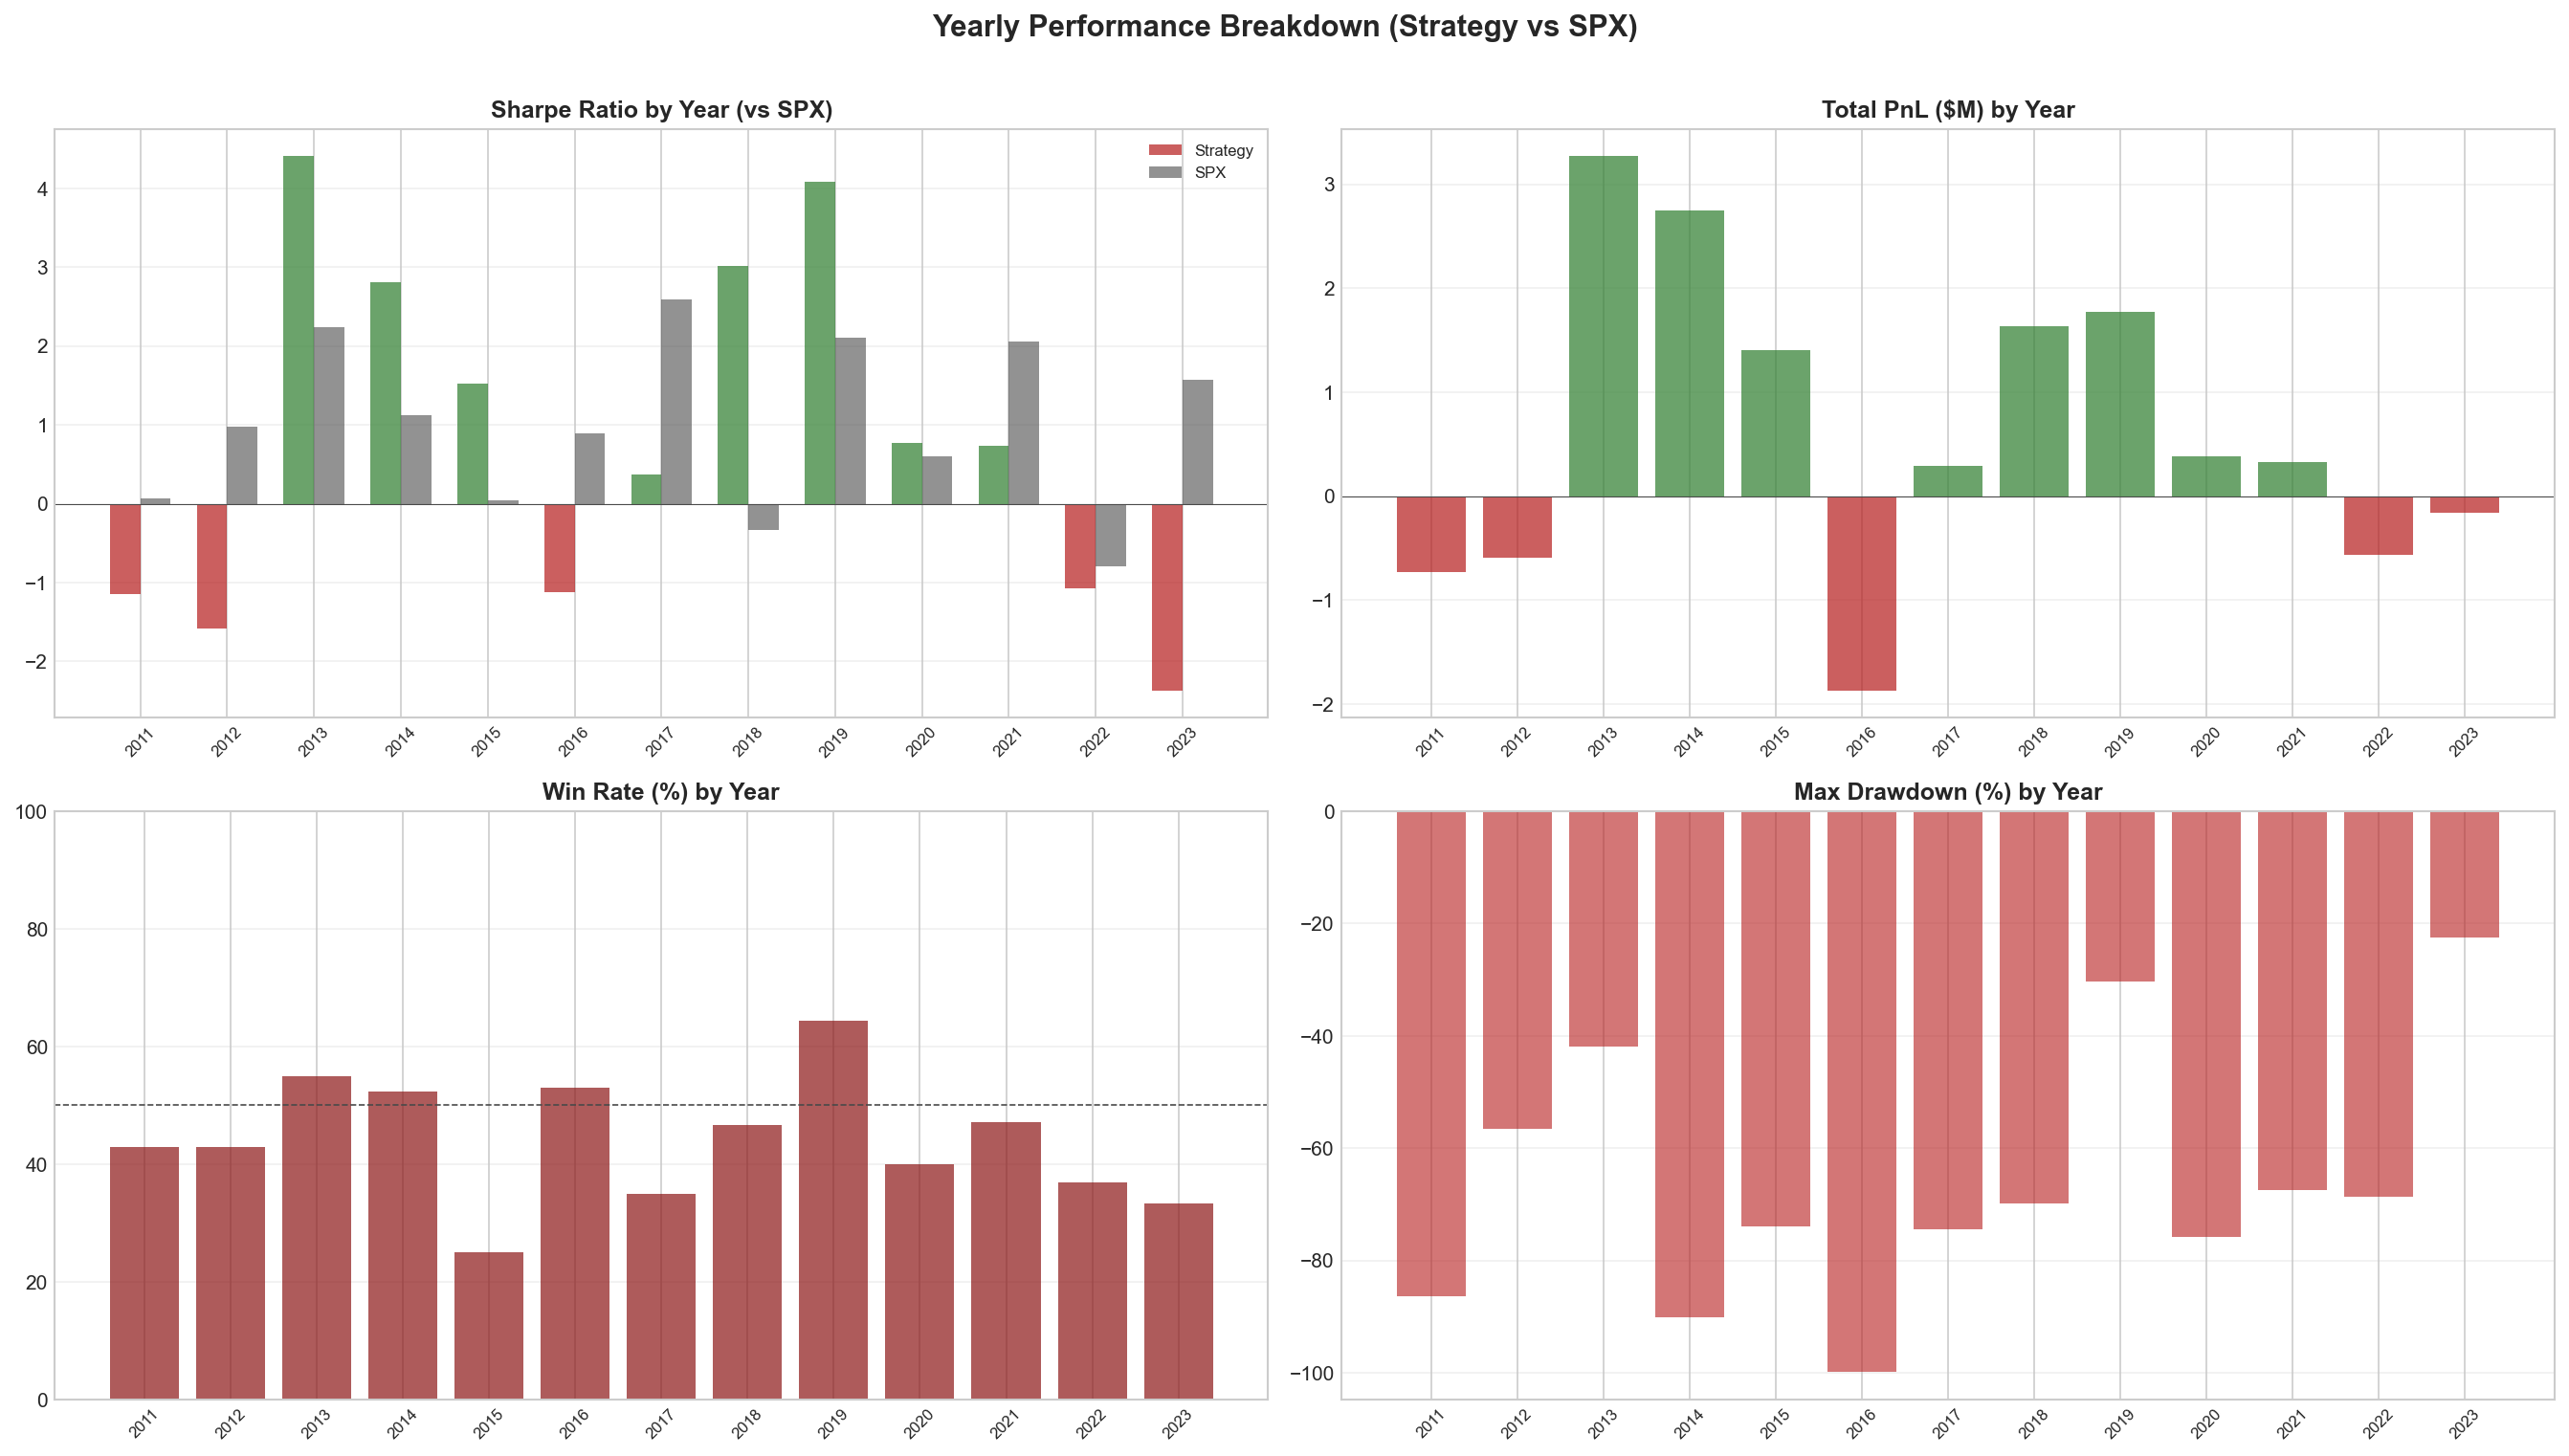
\includegraphics[width=\textwidth]{20_yearly_breakdown.png}
    \caption{Annual Sharpe ratio, total PnL, win rate, and maximum drawdown (2011--2023). The strategy is profitable in 11 of 13 calendar years, with \$26.04\,M cumulative PnL.}
    \label{fig:yearly}
\end{figure}


%%%%%%%%%%%%%%%%%%%%%%%%%%%%%%%%%%%%%%%%%%%%%%%%%%%%%%%%%%%%%%%
\section{Conclusion}
%%%%%%%%%%%%%%%%%%%%%%%%%%%%%%%%%%%%%%%%%%%%%%%%%%%%%%%%%%%%%%%

\subsection{Summary of Findings}

We demonstrate that the variance risk premium, defined as the spread between implied and forecast realized volatility, contains systematic, economically significant alpha in the SPX weekly options market.
Our core VRP signal, combined with a 25\% per-trade stop-loss, produces a Sharpe ratio of 1.10 over the 2011--2023 sample period, generating \$26.04\,M in cumulative PnL across 140 trades on \$1\,M notional capital.
The principal findings are as follows:
\begin{enumerate}[nosep]
    \item The Variance Swap (MFIV) signal delivers superior risk-adjusted performance relative to the ATM~IV baseline, with a Sharpe ratio of 1.26 versus 1.10 and cumulative PnL of \$37.21\,M versus \$26.04\,M, consistent with the theoretical advantages of model-free implied variance.
    \item The logistic regression RV forecast (optimized at $K{=}8$ quantile buckets) achieves a Sharpe ratio of 1.32 and \$26.18\,M in cumulative PnL.
    \item The strategy remains profitable out-of-sample (Sharpe 0.48, \$6.27\,M PnL), providing evidence against in-sample overfitting.
    \item The strategy generates positive PnL during every major stress episode in our sample, with a full-sample maximum drawdown of 83.9\%.
    \item Profitability is maintained across all volatility regimes and in both FOMC and non-FOMC windows.
    \item Results are robust to parameter variation in threshold, transaction cost, and holding period; the block-bootstrap yields $P(\text{Sharpe} > 0) = 100.0\%$.
\end{enumerate}

\subsection{Limitations}

\paragraph{Tail Risk and Drawdown Magnitude.}
The maximum drawdown of 83.9\% is substantial and reflects the inherent concavity of the short-volatility payoff profile.
While the 25\% per-trade stop-loss caps individual losses, we assume that the stop is executable at the specified level; in practice, gap openings and liquidity withdrawal during stress events could result in materially worse execution.

\paragraph{Out-of-Sample Decay.}
The meaningful decline in Sharpe ratio from the in-sample period (1.69) to the out-of-sample period (0.48) warrants scrutiny.
While the signal remains profitable, the decay may reflect structural changes in the volatility market, including the proliferation of short-volatility products, increased competition for the VRP, and the unusual macro regimes of 2020--2023.

\paragraph{Simplified Delta Hedging.}
Our daily delta-hedging simulation does not account for intraday gamma exposure or discrete rebalancing costs.
During rapid market moves, the actual hedging loss may exceed the simulated loss, particularly for short-dated options where gamma is concentrated near expiry.
A higher-fidelity simulation incorporating intraday rebalancing would provide a more conservative performance estimate.

\paragraph{Single Underlying.}
The strategy is evaluated exclusively on SPX index options.
Extending the framework to a diversified universe of liquid single-name or ETF options could improve capacity, reduce concentration risk, and provide a more complete assessment of the VRP as a cross-sectional phenomenon.

\subsection{Extensions and Future Work}

Several avenues for improvement merit investigation:
\begin{enumerate}[nosep]
    \item \textbf{Regime-Conditional Entry}: Condition trade entry on trailing realized volatility regime or macro state variables to concentrate exposure in environments where the VRP is most reliably harvested.
    \item \textbf{Dynamic Position Sizing}: Replace fixed notional sizing with Kelly-criterion or risk-parity methods that cap leverage at $2$--$5\times$ and adapt to prevailing volatility.
    \item \textbf{Intraday Delta Hedging}: Rebalance the delta hedge at higher frequency (e.g., hourly) to reduce gamma exposure during volatile sessions and provide a more realistic accounting of hedging costs.
    \item \textbf{Cross-Sectional Extension}: Apply the VRP signal across a panel of liquid equity options, diversifying idiosyncratic risk and expanding strategy capacity.
    \item \textbf{Machine Learning RV Forecasts}: Augment or replace the linear HAR/GARCH ensemble with recurrent neural networks, gradient-boosted trees, or transformer architectures that may better capture regime transitions and nonlinear volatility dynamics.
\end{enumerate}

\subsection{Concluding Remarks}

The variance risk premium is a well-documented, economically grounded source of returns in equity option markets.
Our results confirm that it can be harvested systematically through a transparent, rule-based signal after accounting for realistic transaction costs and risk management constraints.
However, the strategy's inherently concave payoff profile, characterized by frequent moderate gains and occasional severe losses, demands disciplined risk management.
A production deployment would incorporate hard leverage limits, regime-aware position sizing, intraday hedging, and a diversified underlying universe to manage tail risk.
The VRP is real and exploitable, but harvesting it reliably requires a thorough understanding of its time-varying nature and the structural risks of short-volatility exposure.


%%%%%%%%%%%%%%%%%%%%%%%%%%%%%%%%%%%%%%%%%%%%%%%%%%%%%%%%%%%%%%%
% REFERENCES
%%%%%%%%%%%%%%%%%%%%%%%%%%%%%%%%%%%%%%%%%%%%%%%%%%%%%%%%%%%%%%%
\newpage
\bibliographystyle{plainnat}

\begin{thebibliography}{20}

\bibitem[Andersen et~al.(2003)]{andersen2003modeling}
Andersen, T.~G., Bollerslev, T., Diebold, F.~X., and Labys, P. (2003).
\newblock Modeling and Forecasting Realized Volatility.
\newblock \textit{Econometrica}, 71(2):579--625.

\bibitem[Bakshi et~al.(2003)]{bakshi2003stock}
Bakshi, G., Kapadia, N., and Madan, D. (2003).
\newblock Stock Return Characteristics, Skew Laws, and the Differential Pricing of Individual Equity Options.
\newblock \textit{Review of Financial Studies}, 16(1):101--143.

\bibitem[Bollerslev et~al.(2009)]{bollerslev2009expected}
Bollerslev, T., Tauchen, G., and Zhou, H. (2009).
\newblock Expected Stock Returns and Variance Risk Premia.
\newblock \textit{Review of Financial Studies}, 22(11):4463--4492.

\bibitem[Bondarenko(2003)]{bondarenko2003why}
Bondarenko, O. (2003).
\newblock Why Are Put Options So Expensive?
\newblock Working Paper, University of Illinois at Chicago.

\bibitem[Breeden and Litzenberger(1978)]{breeden1978prices}
Breeden, D.~T. and Litzenberger, R.~H. (1978).
\newblock Prices of State-Contingent Claims Implicit in Option Prices.
\newblock \textit{Journal of Business}, 51(4):621--651.

\bibitem[Carr and Madan(1998)]{carr1998towards}
Carr, P. and Madan, D. (1998).
\newblock Towards a Theory of Volatility Trading.
\newblock In Jarrow, R., editor, \textit{Volatility: New Estimation Techniques for Pricing Derivatives}, pages 417--427. Risk Books.

\bibitem[Carr and Wu(2009)]{carr2009variance}
Carr, P. and Wu, L. (2009).
\newblock Variance Risk Premiums.
\newblock \textit{Review of Financial Studies}, 22(3):1311--1341.

\bibitem[Corsi(2009)]{corsi2009simple}
Corsi, F. (2009).
\newblock A Simple Approximate Long-Memory Model of Realized Volatility.
\newblock \textit{Journal of Financial Econometrics}, 7(2):174--196.

\bibitem[Demeterfi et~al.(1999)]{demeterfi1999more}
Demeterfi, K., Derman, E., Kamal, M., and Zou, J. (1999).
\newblock More Than You Ever Wanted to Know About Volatility Swaps.
\newblock Goldman Sachs Quantitative Strategies Research Notes.

\bibitem[Drechsler and Yaron(2011)]{drechsler2011whats}
Drechsler, I. and Yaron, A. (2011).
\newblock What's Vol Got to Do with It.
\newblock \textit{Review of Financial Studies}, 24(1):1--45.

\bibitem[Gatheral(2006)]{gatheral2006volatility}
Gatheral, J. (2006).
\newblock \textit{The Volatility Surface: A Practitioner's Guide}.
\newblock Wiley Finance.

\bibitem[Hansen et~al.(2012)]{hansen2012realized}
Hansen, P.~R., Huang, Z., and Shek, H.~H. (2012).
\newblock Realized GARCH: A Joint Model for Returns and Realized Measures of Volatility.
\newblock \textit{Journal of Applied Econometrics}, 27(6):877--906.

\bibitem[Augustin et~al.(2021)]{augustin2021volmageddon}
Augustin, P., Cheng, I.-H., and Van den Bergen, L. (2021).
\newblock Volmageddon and the Failure of Short Volatility Products.
\newblock \textit{Financial Analysts Journal}, 77(3).
\newblock \url{https://rpc.cfainstitute.org/research/financial-analysts-journal/2021/volmageddon-failure-short-volatility-products}.

\end{thebibliography}


%%%%%%%%%%%%%%%%%%%%%%%%%%%%%%%%%%%%%%%%%%%%%%%%%%%%%%%%%%%%%%%
% APPENDIX
%%%%%%%%%%%%%%%%%%%%%%%%%%%%%%%%%%%%%%%%%%%%%%%%%%%%%%%%%%%%%%%
\newpage
\appendix
\section{Additional Figures}

\begin{figure}[H]
    \centering
    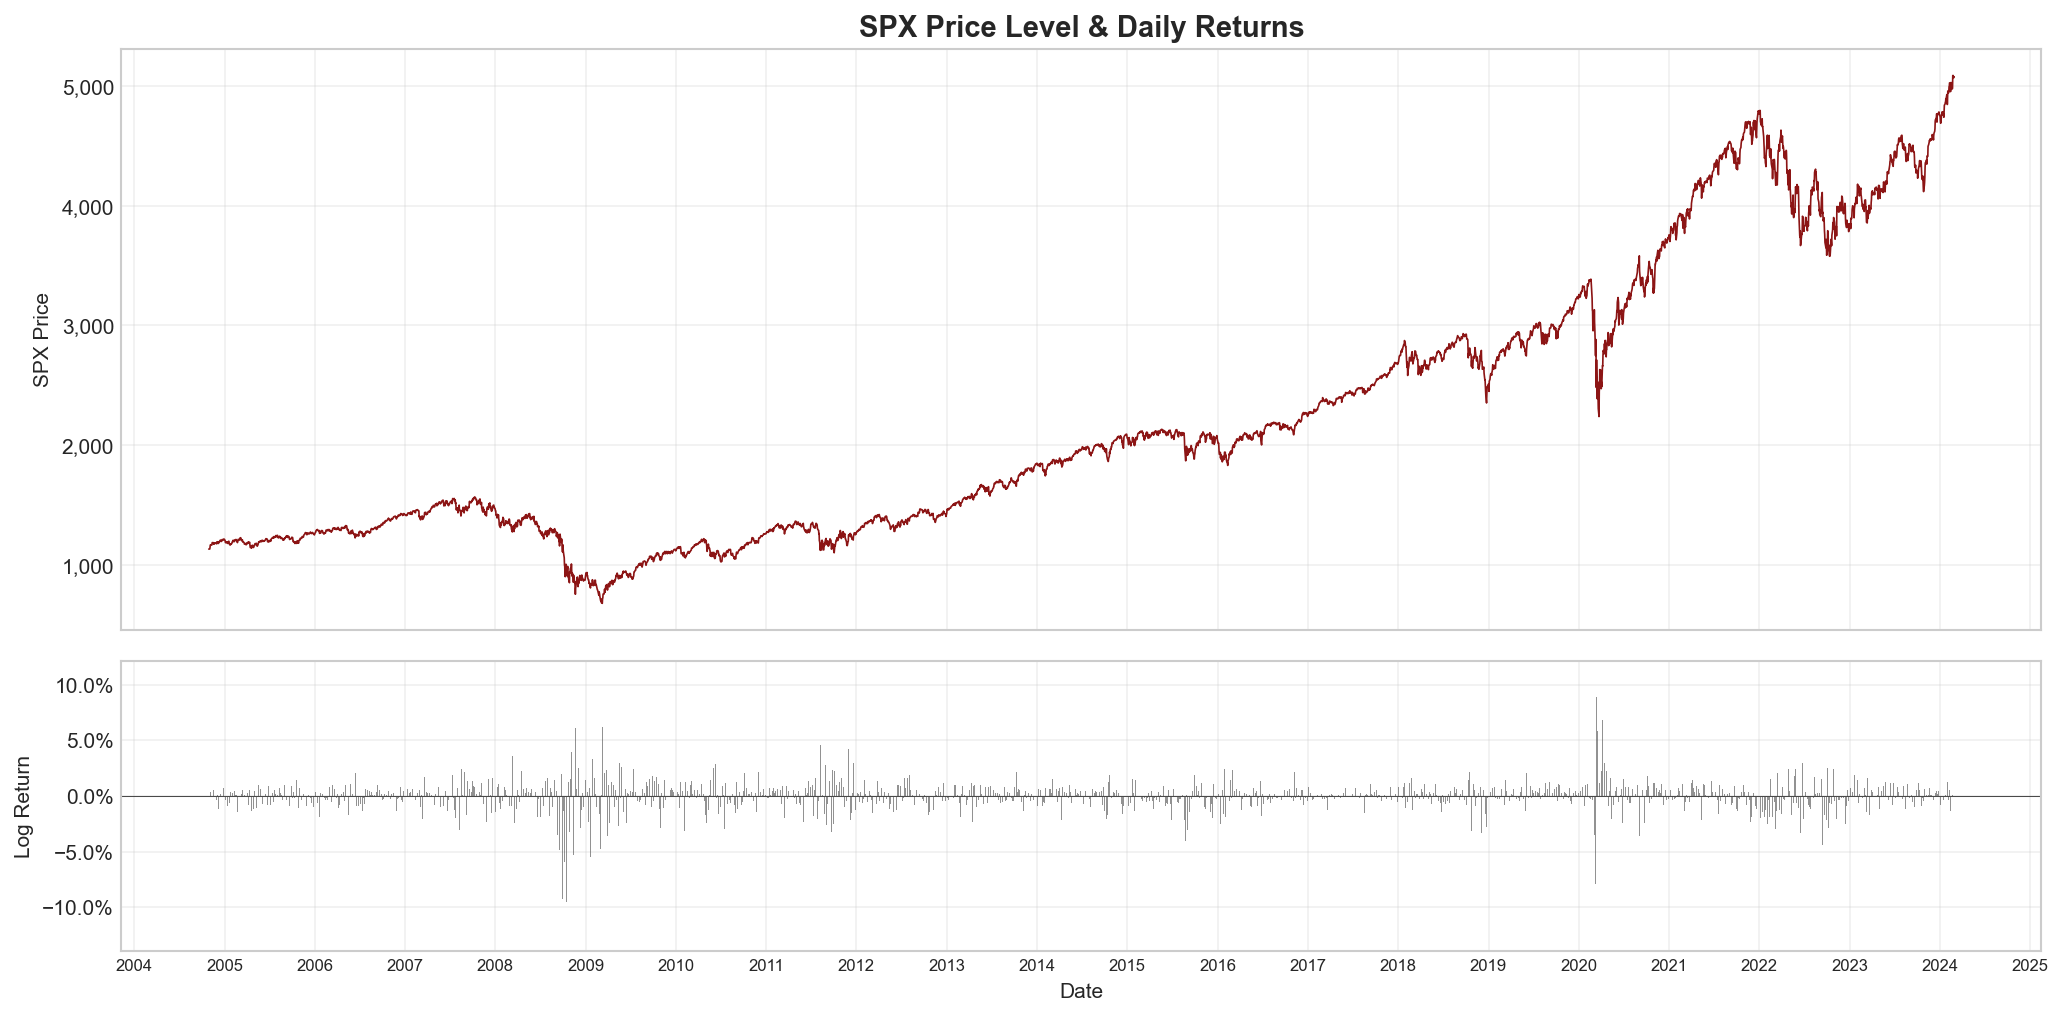
\includegraphics[width=\textwidth]{01_spx_price_returns.png}
    \caption{SPX price history and log return distribution (2005--2023).}
\end{figure}

\begin{figure}[H]
    \centering
    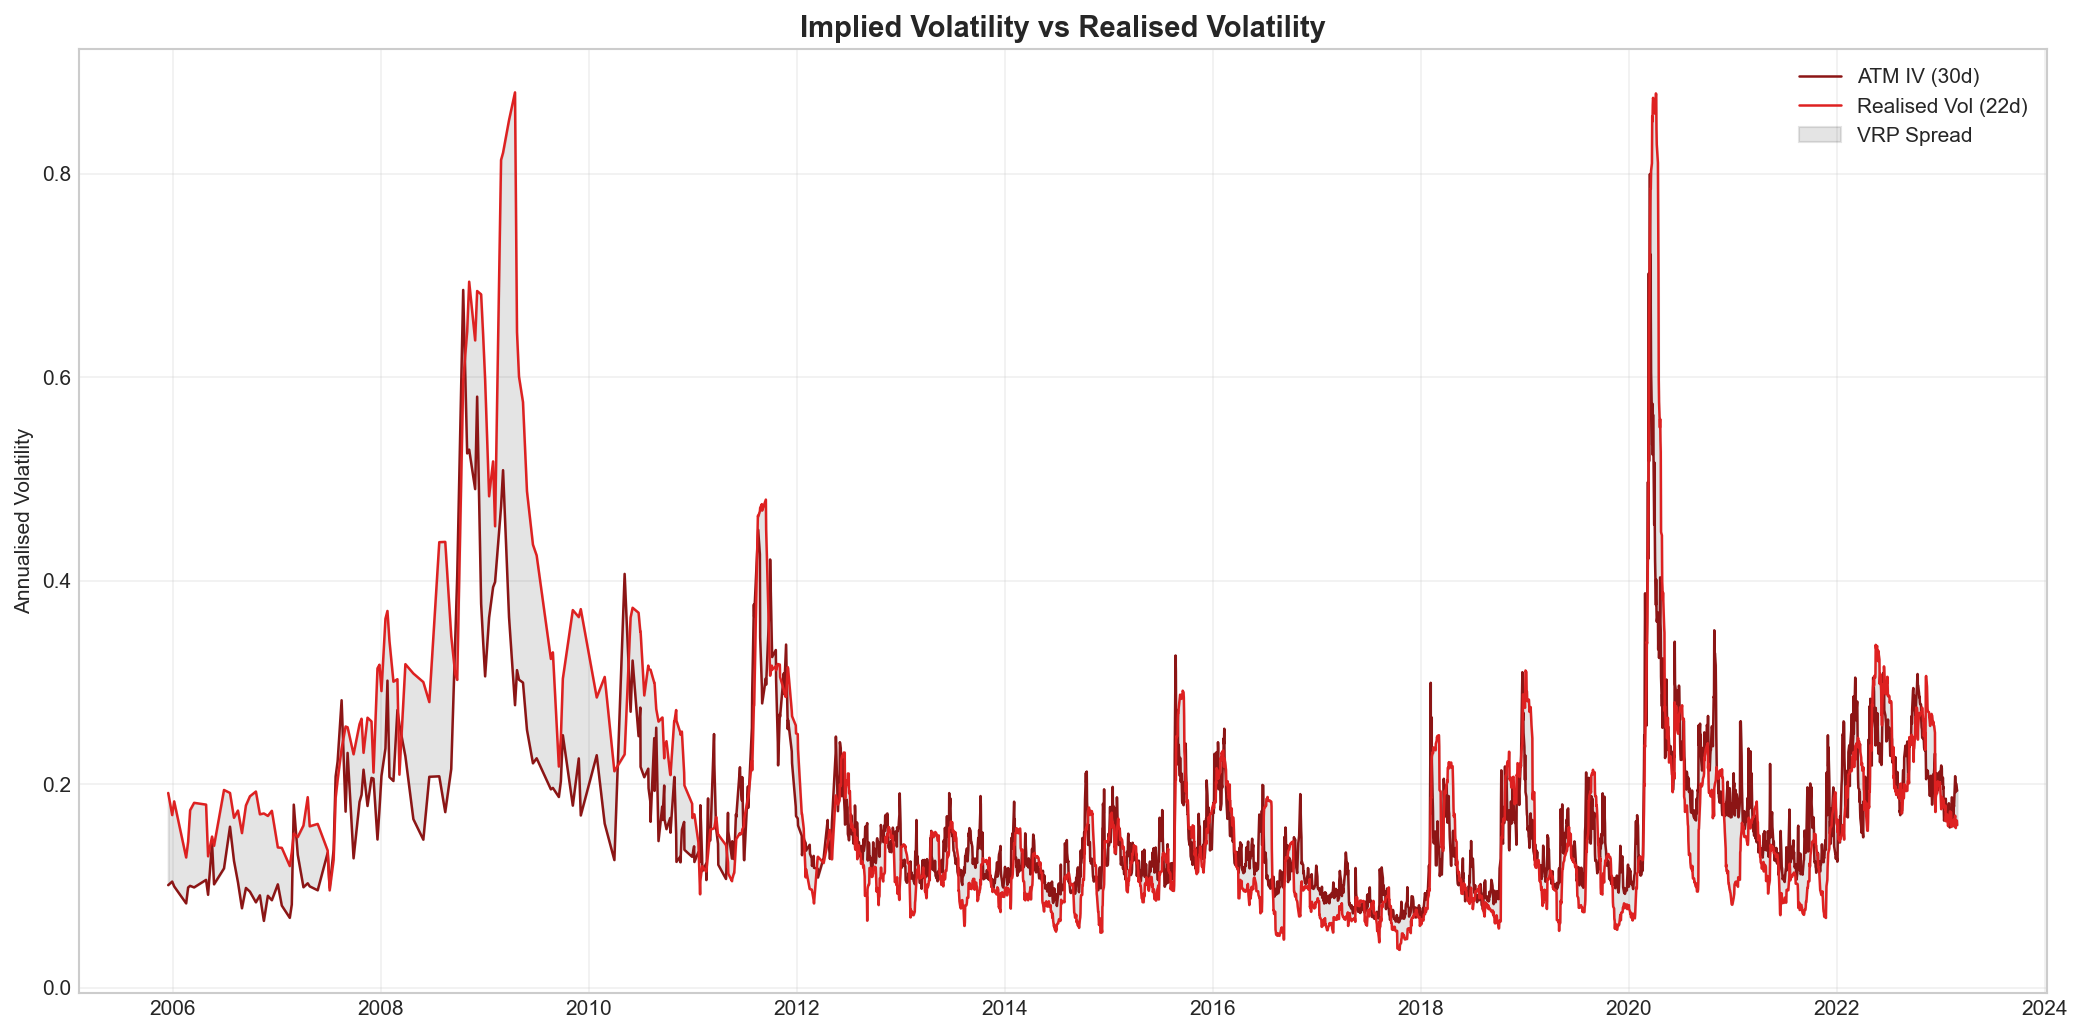
\includegraphics[width=\textwidth]{03_iv_vs_rv.png}
    \caption{ATM implied volatility versus realized volatility time series and their spread.}
\end{figure}

\begin{figure}[H]
    \centering
    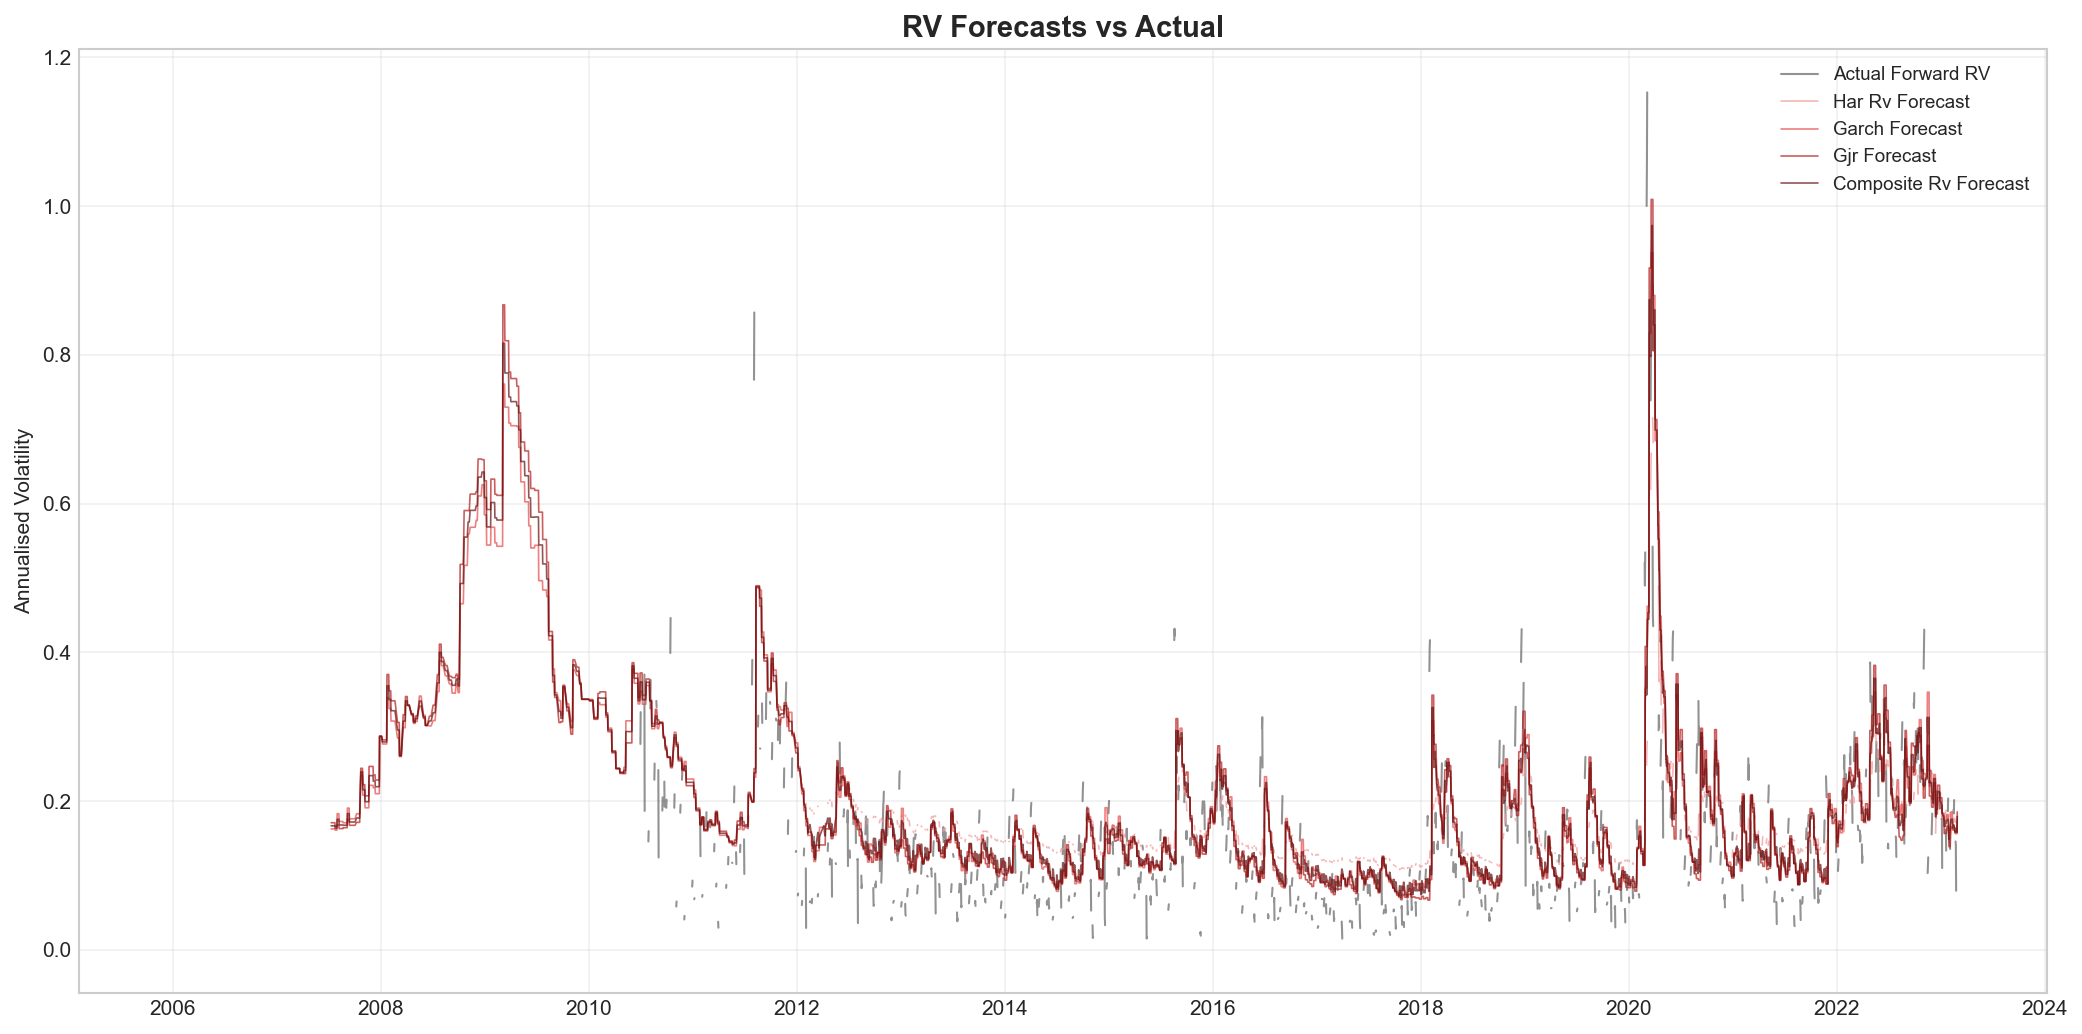
\includegraphics[width=\textwidth]{04_rv_forecasts.png}
    \caption{Rolling RV forecast models: HAR-RV, GARCH(1,1), GJR-GARCH(1,1), and composite forecast.}
\end{figure}

\begin{figure}[H]
    \centering
    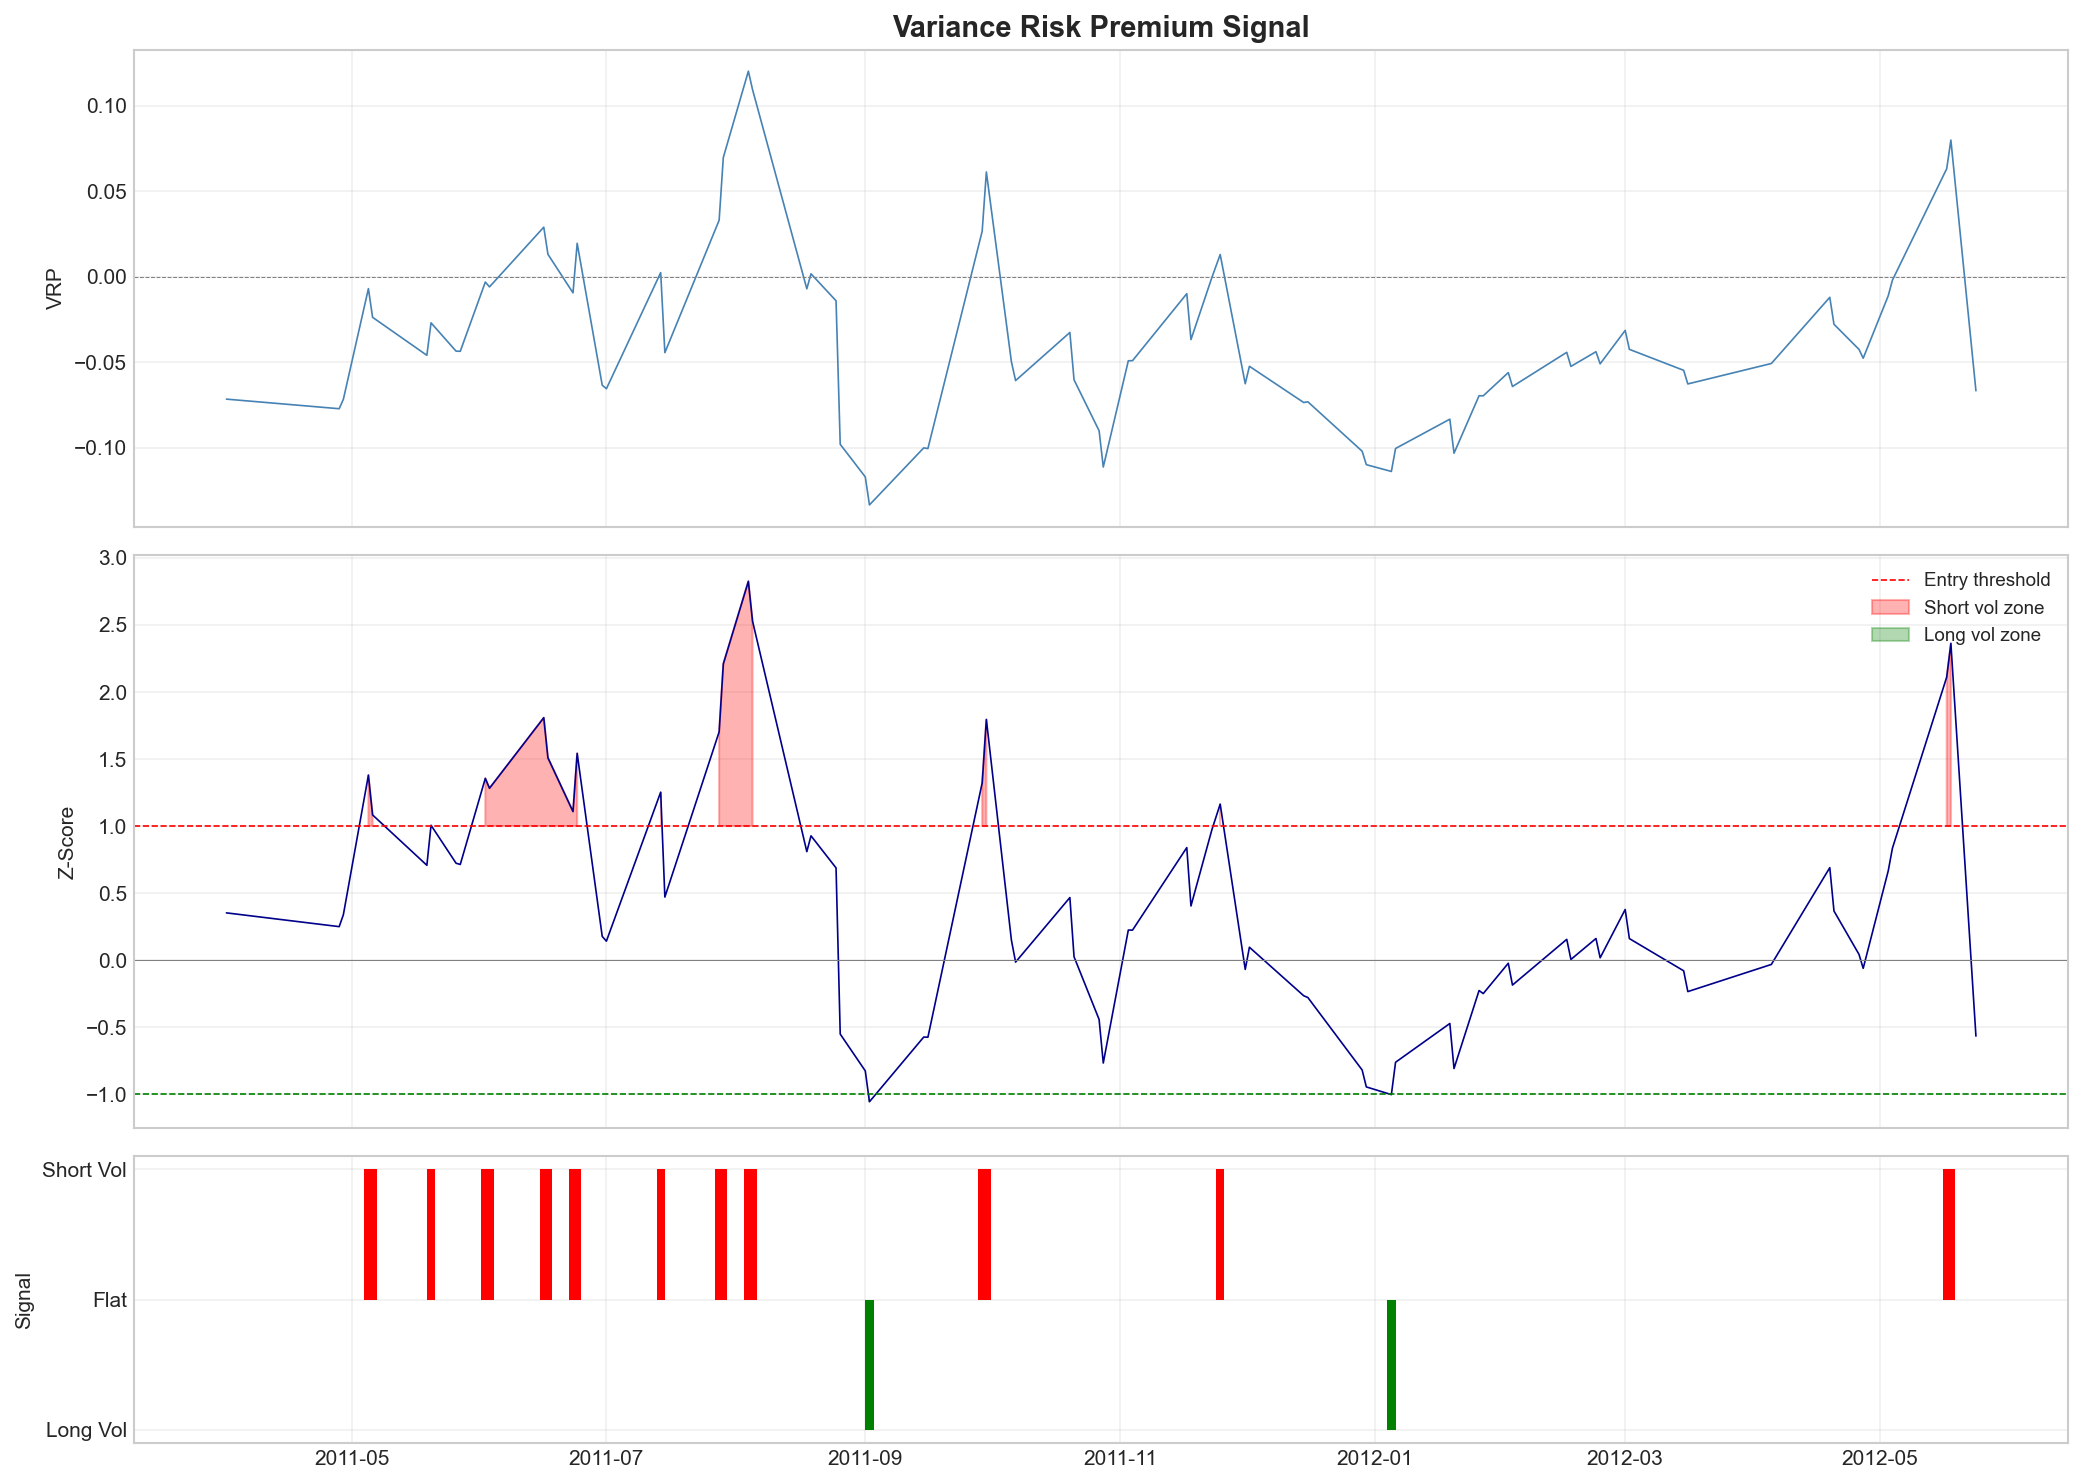
\includegraphics[width=\textwidth]{05_vrp_signal.png}
    \caption{VRP signal z-score and discrete trading signals over time.}
\end{figure}

\begin{figure}[H]
    \centering
    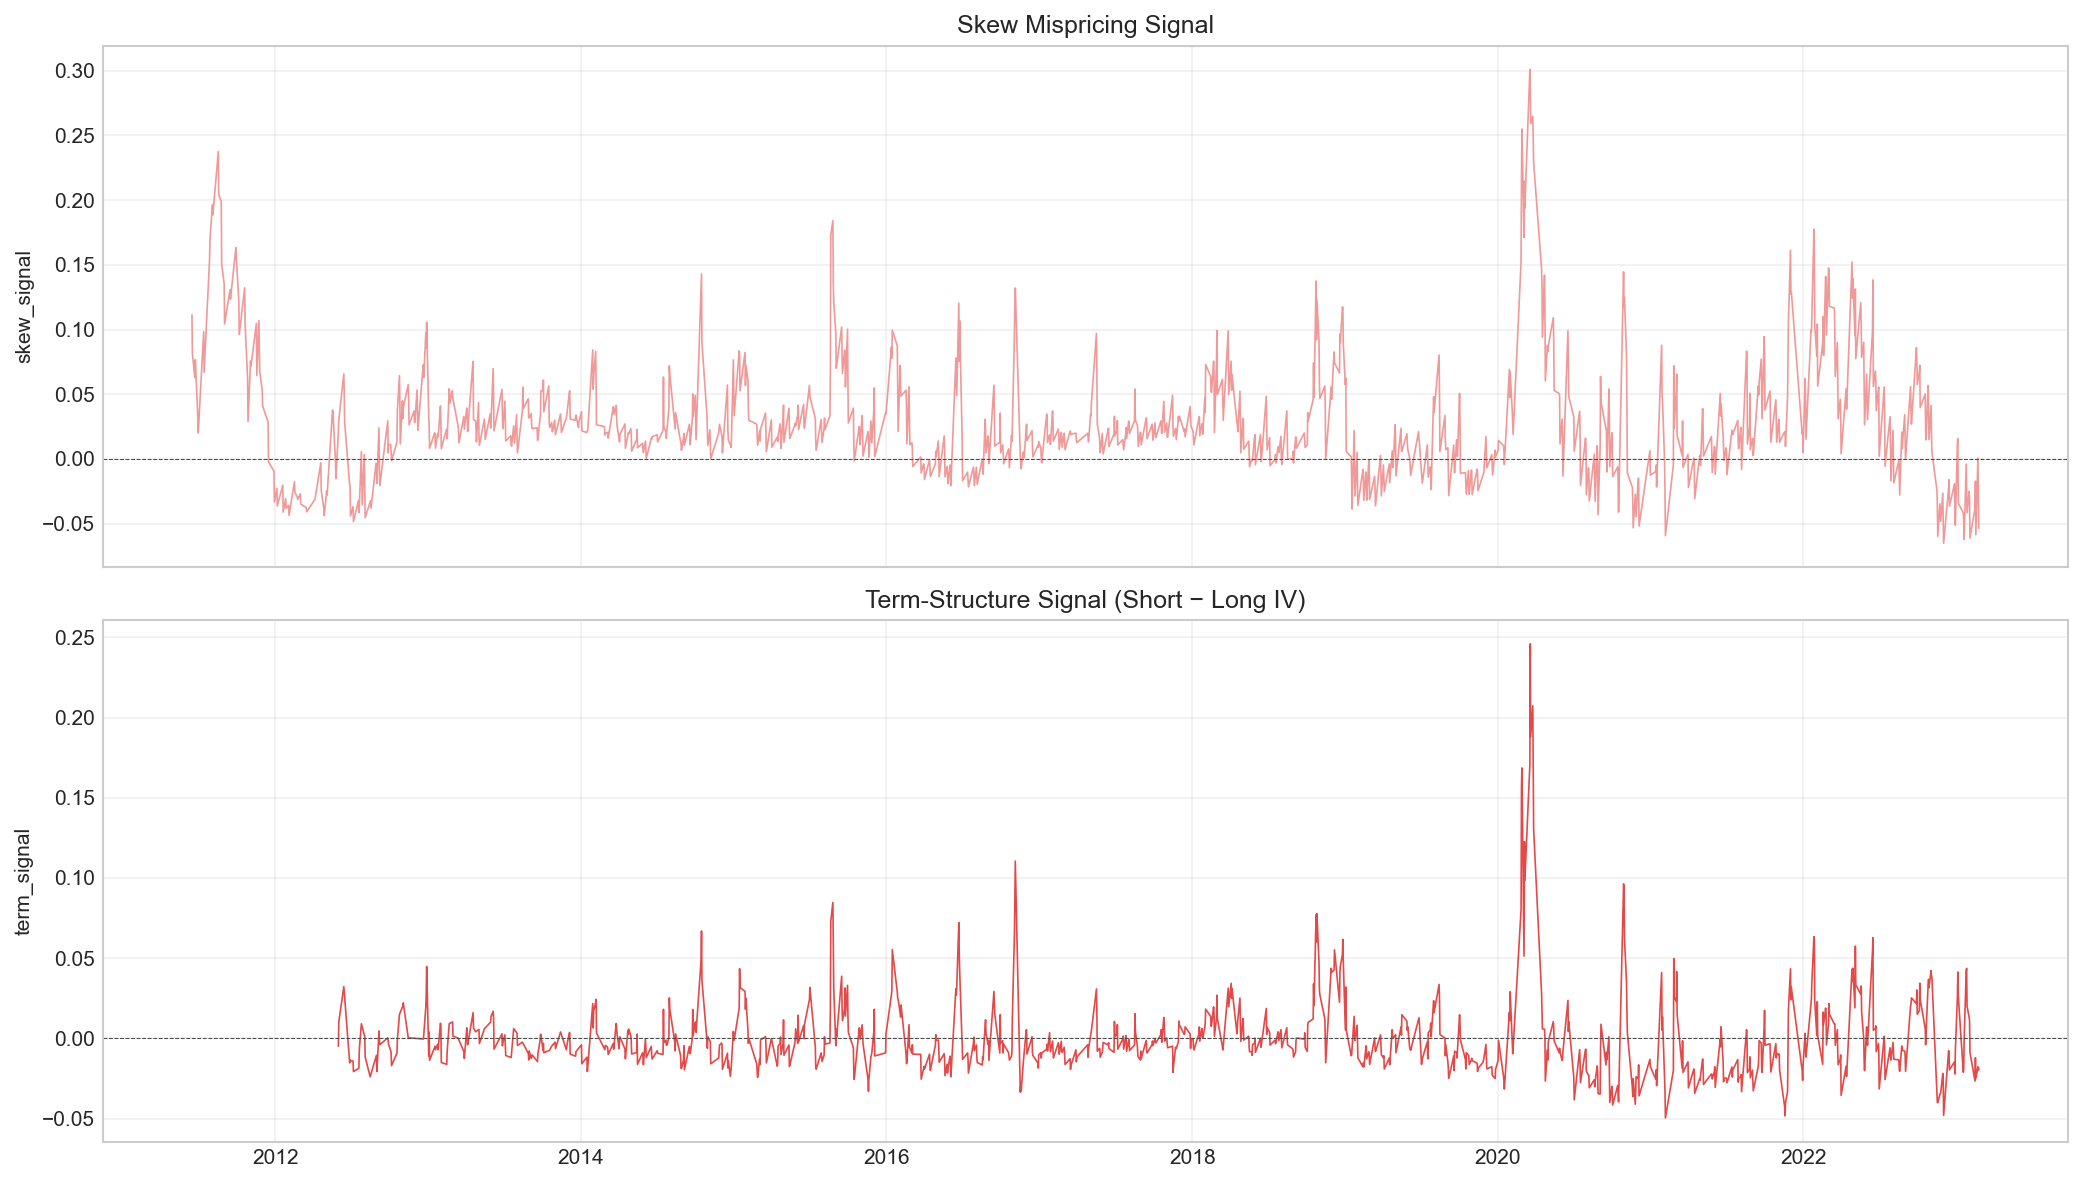
\includegraphics[width=\textwidth]{06_surface_signals.png}
    \caption{Implied volatility skew and term-structure surface signals.}
\end{figure}

\begin{figure}[H]
    \centering
    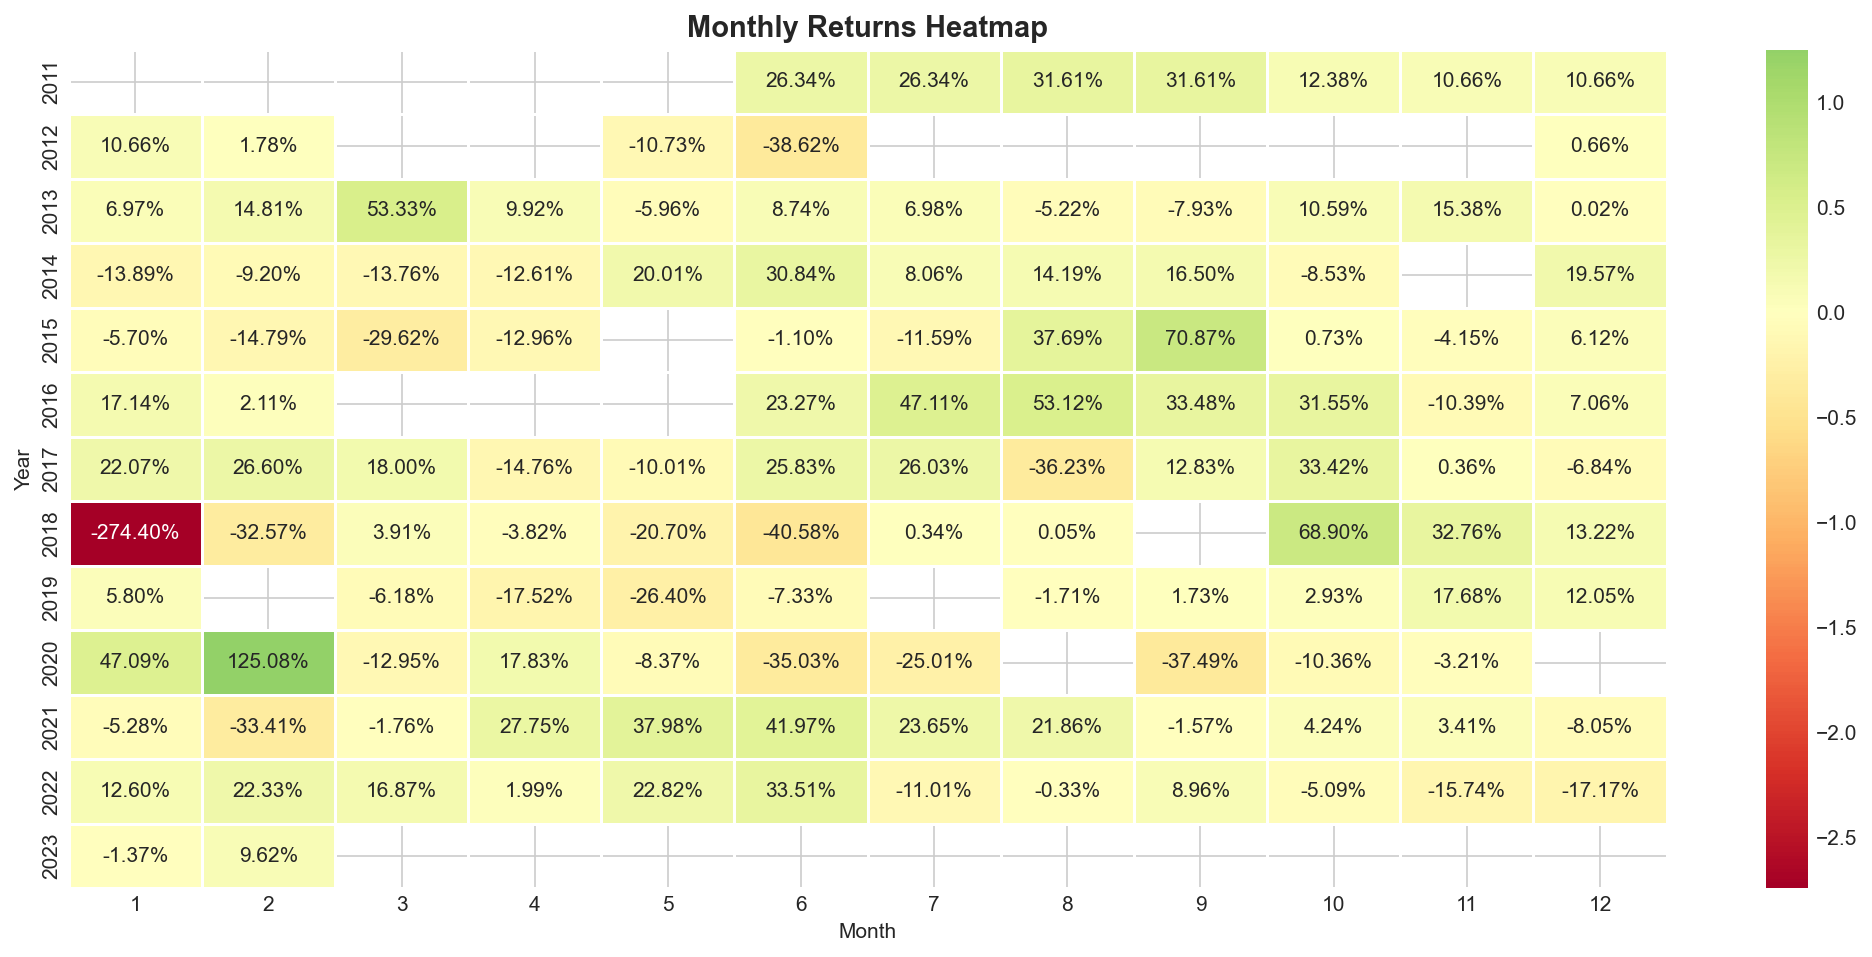
\includegraphics[width=\textwidth]{09_monthly_returns.png}
    \caption{Monthly return heatmap.}
\end{figure}

\begin{figure}[H]
    \centering
    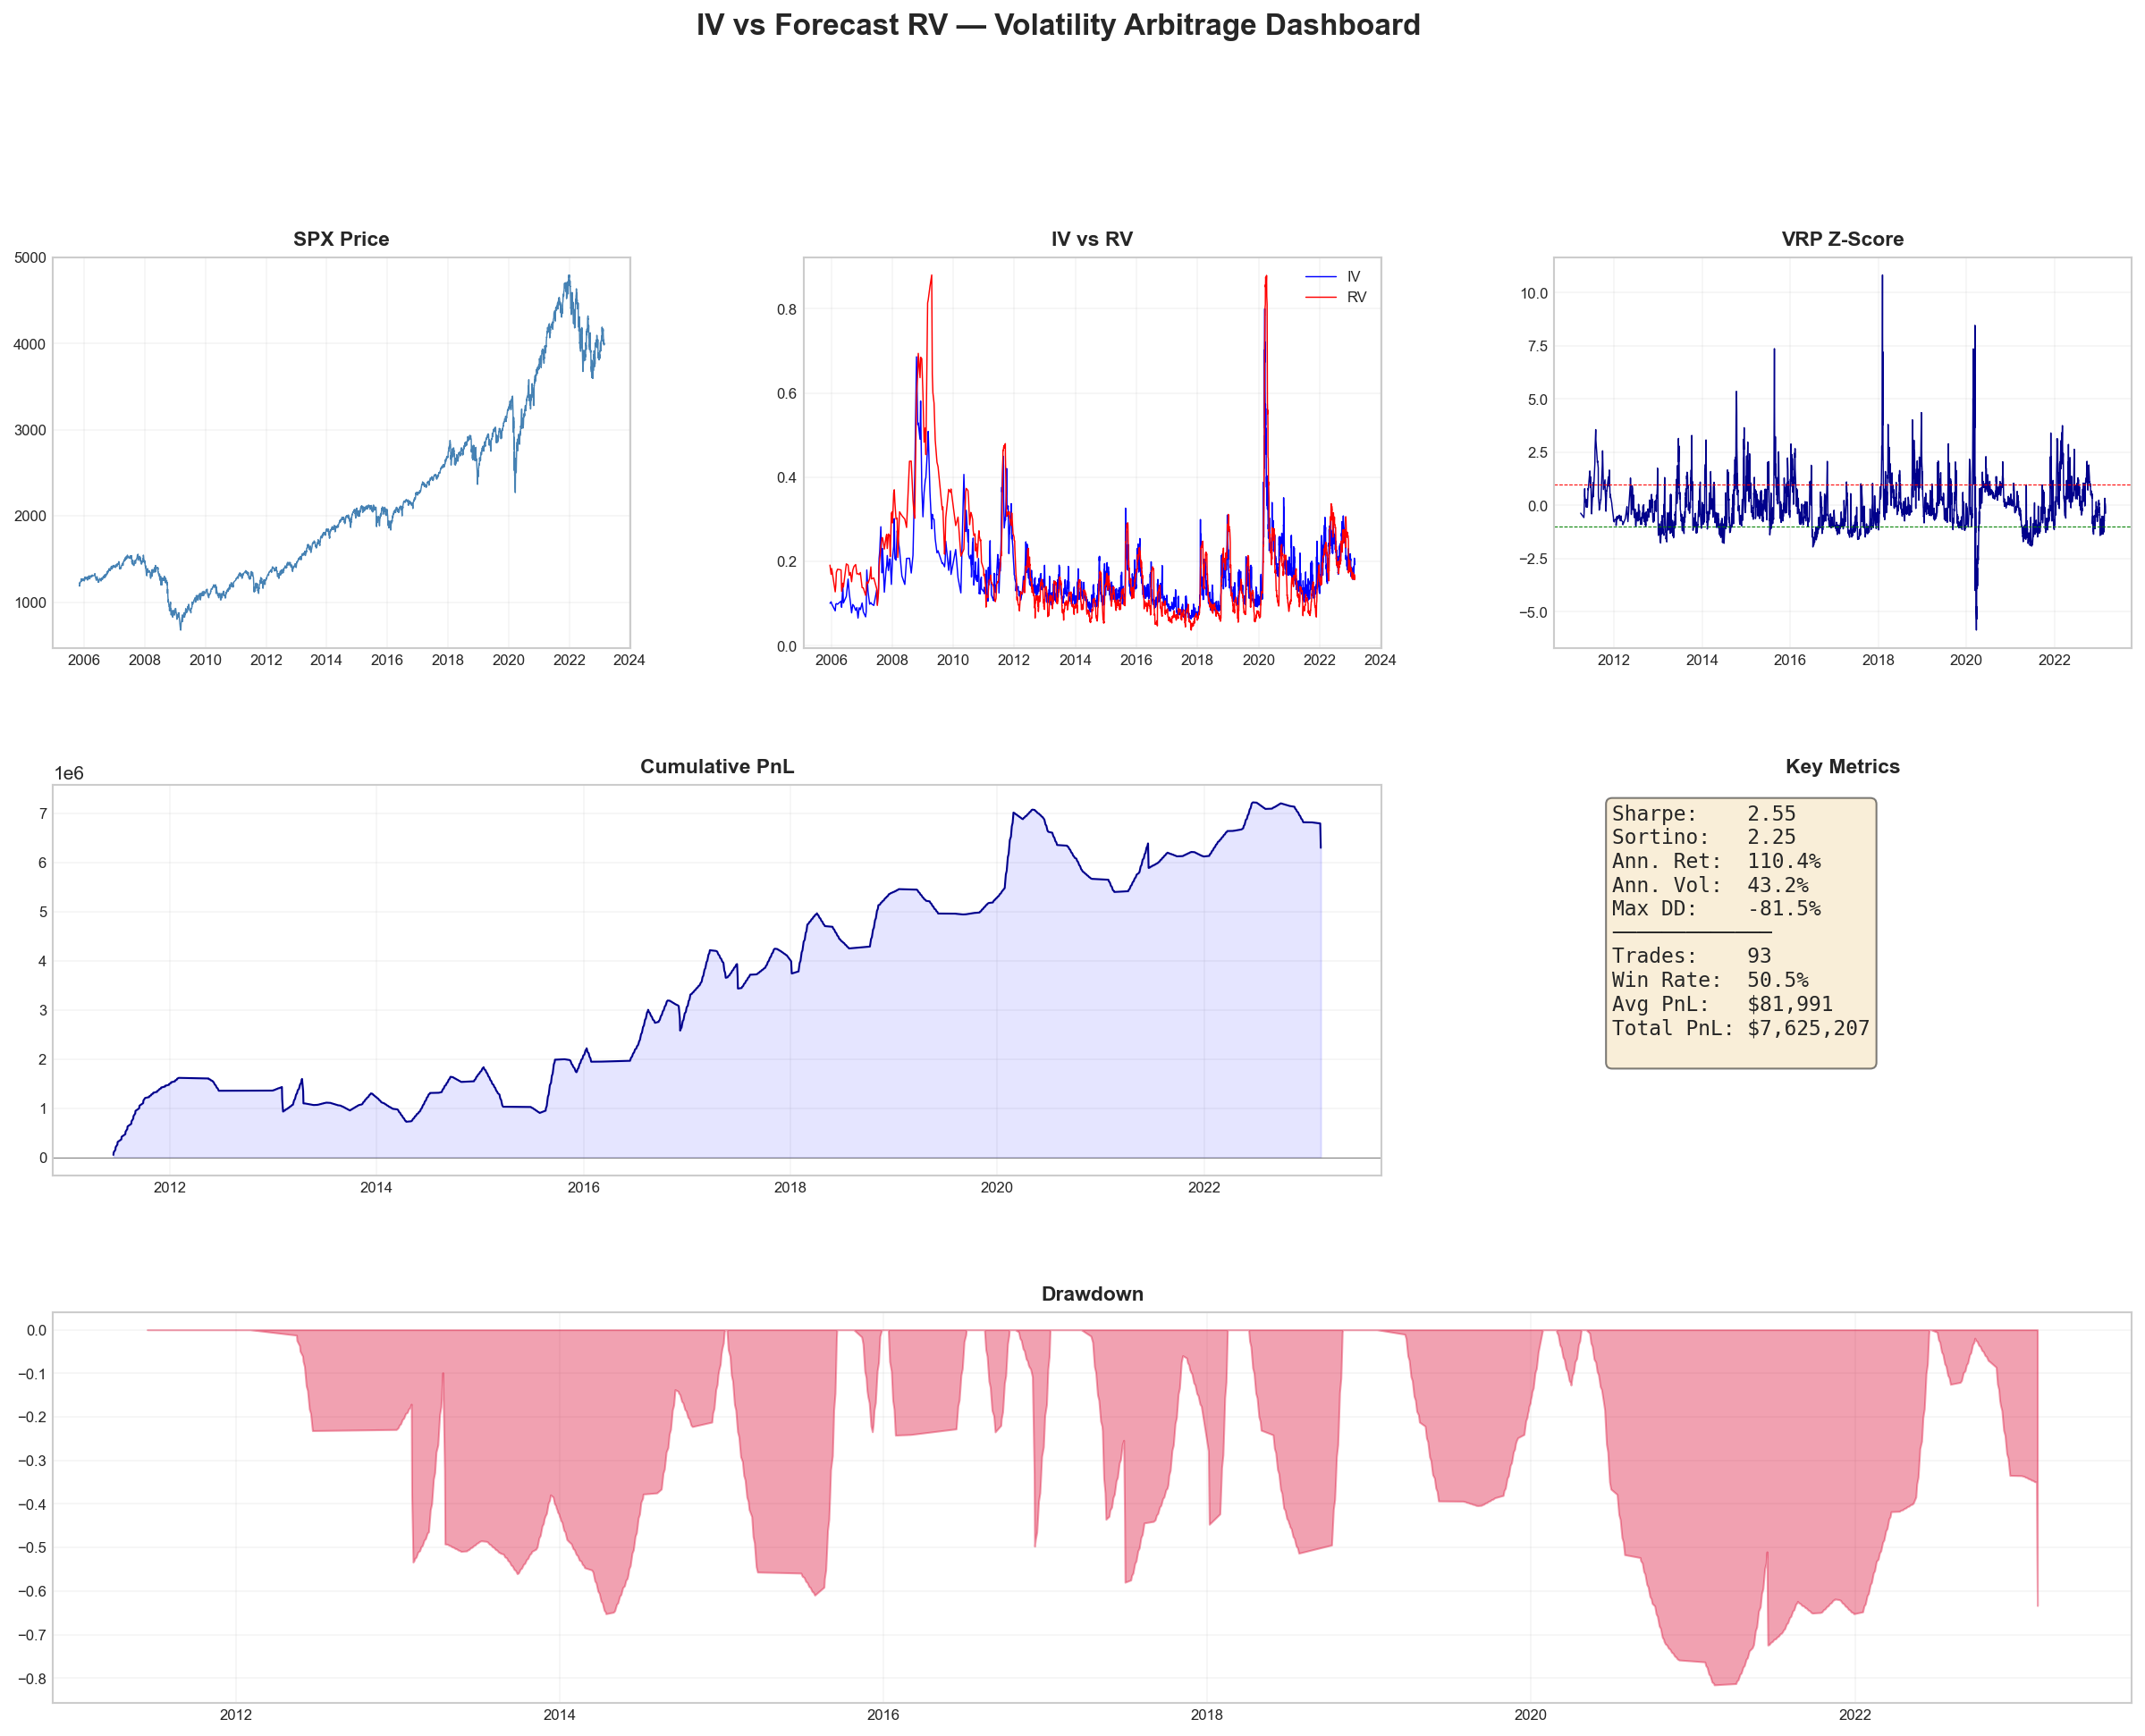
\includegraphics[width=\textwidth]{12_summary_dashboard.png}
    \caption{Summary performance dashboard.}
\end{figure}

\end{document}
